%
% Modelo para relat￳rio da disciplina de Projecto de Engenharia Informatica
% do MEI.
%
% Incorpora elementos impostos pelo Regulamento de Estudos Pos-Graduados da
% Universidade de Lisboa (Deliberacao 1506/2006 - Diario da Repblica, 2.a s←rie 
% - n.o 209 - 30 de Outubro de 2006)
%
\documentclass[12pt,openright,twoside]{report}
\usepackage[hide]{chato-notes}
\usepackage[utf8]{inputenc}
% Quem tiver problemas com os acentos, trocar utf8 por latin1

%\usepackage{setspace}
\usepackage[portuguese,english]{babel}
\usepackage{times}
\usepackage{url}
\usepackage{graphicx}
\usepackage{mdwlist}
\usepackage[nottoc]{tocbibind}
\usepackage{csquotes}
\usepackage[table,hyperref,x11names]{xcolor}
\usepackage{array,booktabs}
\usepackage{multirow}

\usepackage{dialogue}
%To get figures and tables side by side
\usepackage{floatrow}
\newfloatcommand{capbtabbox}{table}[][\FBwidth]
% end figures and tables side by side

%footnote in tables 
\usepackage{threeparttable}
%end footnote in tables

% Indice remissivo
\usepackage{makeidx}
\makeindex

%%%%%%%%%%%%%%%%%% BIG O 
\usepackage{amsmath}
\newcommand{\BigO}[1]{\ensuremath{\operatorname{O}\bigl(#1\bigr)}}
%%%%%%%%%%%%%% BIG O
%quotes
\usepackage{epigraph}
\usepackage{attrib}
\usepackage{titlesec}

%\titlespacing{\subsubsection}{0pt}{0pt}{0pt}
\titleformat{\subsubsection}[runin]{\normalfont\bfseries}{\thesubsection.}{3pt}{}


\usepackage[nomain,acronym,xindy,nonumberlist]{glossaries}
\newacronym{sdn}{SDN}{Software Defined Network}

\newacronym{nib}{NIB}{Network Information Base}

\newacronym{wan}{WAN}{Wide Area Network}

\newacronym{nos}{NOS}{Network Operating System}

\newacronym{os}{OS}{Operating System}

\newacronym{onf}{ONF}{Open Network Foundation}

\newacronym{of}{OF}{OpenFlow}

\newacronym{fifo}{FIFO}{First In,First Out}

\newacronym{smr}{SMR}{State Machine Replication}

\newacronym{arp}{ARP}{Address Resolution Protocol}
\newacronym{api}{API}{Application Programming Interface}
\newacronym{lru}{LRU}{Least Recently Used} 
\newacronym{ip}{IP}{Internet Protocol}
\newacronym{icmp}{ICMP}{Internet Control Message Protocol} 
\newacronym{ipv6}{IPv6}{Internet Protocol version 6}
\newacronym{vlan}{VLAN}{Virtual Local Area Network} 
\newacronym{mac}{MAC}{Media Access Control}


\newacronym{rest}{REST}{Representational State Transfer} 
\newacronym{vip}{VIP}{Virtual Enpoint Internet Protocol} 
\newacronym{rpc}{RPC}{Remote Procedure Call} 
\newacronym{sql}{SQL}{Structured Query Language} 

\newacronym{tcp}{TCP}{Transmission Control Protocol}
\newacronym{rcp}{RCP}{Routing Control Platform}
\newacronym{bgp}{BGP}{Border Gateway Protocol}
\newacronym{as}{AS}{Autonomous System}
\newacronym{ibgp}{iBGP}{interior Border Gateway Protocol}
\newacronym{url}{URL}{Uniform Resource Locator}
\newacronym{dhcp}{DHCP}{Dynamic Host Configuration Protocol}
\newacronym{http}{HTTP}{HyperText Transport Protocol} 
\makeglossary  

% Links
\usepackage{hyperref}

% Package para cabecalhos
\usepackage{fancyhdr}
\usepackage{lastpage}

\usepackage[font={small}]{caption}
\usepackage{subcaption}
\usepackage[sorting=none,  isbn=false,
url=false, doi=false, eprint=false]{biblatex}

\bibliography{bibliografia,web}
\fancyhf{} %
\lhead{\nouppercase {\leftmark}} %
\rhead{\nouppercase {\bf \thepage}}
\renewcommand{\headrulewidth}{0.1pt}

% Comando para inserir pagina em branco (inserida na numeracao, mas sem
% numero impresso) para quando e' preciso obrigar um capitulo a comecar
% do lado direito (pagina impar)
\newcommand{\LIMPA}{
\newpage
\mbox{}
\thispagestyle{empty}
}

% Igual, mas insere pagina com numero impresso (normalmente nao se usa)
\newcommand{\LIMPAC}{
\newpage
\mbox{}
\thispagestyle{plain}
}


%%%%%%% PERSONAL COMMANDS %%%%%%%%%%%
\newcommand{\distcontrollers}{\cite{:vn, Tootoonchian:2010vy,Koponen:2010th,Yeganeh:2012jm}}
\newcommand{\distcontrollerspaper}{\cite{Tootoonchian:2010vy, Koponen:2010th,Yeganeh:2012jm}}
%END 

\newcommand{\tbl}[2]{\begin{tabular}{#1}#2\end{tabular}}
\newcommand{\ml}[2]{#1 $\pm$ #2} 

%
% ALTERAR AQUI AS INFORMACOES RELATIVAS AO PROJECTO
%
\newcommand{\PEITITULO}{A Consistent and Fault-Tolerant Network
  Information Base for Scalable Software Defined Networks}
\newcommand{\PEIAutor}{Fábio Andrade Botelho}
\newcommand{\PEIAutorNumAluno}{41625}

%Orientador e CoOrientador *sem* titulos (e.g. Prof. Doutor)
\newcommand{\PEIOrientador}{Alysson Neves Bessani}
\newcommand{\PEICoOrientador}{Fernando Manuel Valente Ramos} %se nao se aplicar, nao importa o que aqui esteja

%Se aplicavel, o supervisor pode ter um titulo (Dr., Eng.) colocado aqui
\newcommand{\PEISupervisorInstituicao}{Nome Completo do Supervisor}  %se nao se aplicar, nao importa o que aqui esteja

\newcommand{\PEIAnoLectivo}{2012/2013}
\newcommand{\PEIAno}{2013}

% Comentar/descomentar conforme conveniente
\newcommand{\PEITIPO}{DISSERTA\c{C}\~{A}O }
%\newcommand{\PEITIPO}{PROJECTO }

% Comentar/descomentar conforme conveniente
%\newcommand{\PEIIdiomaTese}{\selectlanguage{portuguese}}
\newcommand{\PEIIdiomaTese}{\selectlanguage{english}}

% Comentar/descomentar conforme conveniente
%\newcommand{\MEIEspecializacao}{Segurança Informática}
%\newcommand{\MEIEspecializacao}{Arquitectura, Sistemas e Redes de Computadores}
%\newcommand{\MEIEspecializacao}{Interac��o e Conhecimento}
%\newcommand{\MEIEspecializacao}{Engenharia de Software }

\usepackage{ifpdf}
\ifpdf
\pdfinfo {
	/Author (\PEIAutor)
	/Title (Projecto em Segurança Informatica)
	/Subject (Segurança Informatica)
	/Keywords (state machine replication, software defined networks)
	/CreationDate (D:20100510104905)
}
\fi

\usepackage[dvips]{geometry}
\geometry{a4paper=true,portrait=true,left=3cm,right=3cm,top=2.5cm,bottom=3.5cm}

\title{\PEITITULO}
\author{\PEIAutor}
%\date{\today}

\begin{document}

%\doublespacing

%Capa e pagina de rosto
\selectlanguage{portuguese}

\pagestyle{empty}

% ----------------------------------------------------------------------
% Capa
\begin{center}
\vspace{3cm}\normalfont\normalfont
\textsc{\huge{Universidade de Lisboa}}\\
\LARGE{Faculdade de Ci\^{e}ncias}\\
\Large{Departamento de Inform\'{a}tica}\\
\vspace{1cm}
\includegraphics[scale=.3]{pic/logo_ul.jpg}\\
%\includegraphics[scale=.6]{pic/logo_fcul.jpg}\\

\vspace{2cm}
\PEIIdiomaTese
\Large{\bf \PEITITULO}\\
\selectlanguage{portuguese}
\vspace{1cm}
%projecto realizado na\\
\vspace{0.7cm}
%\Large{\bf Nome da Instituicao de Acolhimento}\\
%\vspace{0.7cm}
%por\\
\vspace{0.7cm}
\Large{\bf \PEIAutor}\\
\vspace{2.4cm}
\Large{\bf \PEITIPO}\\
\vfill
\Large{MESTRADO EM SEGURANÇA  INFORM\'{A}TICA}\\

\vfill
\PEIAno

\end{center}
\newpage
\mbox{}
\newpage
% Fim da capa
% ----------------------------------------------------------------------

\setcounter{page}{1}
\pagenumbering{roman}

% ----------------------------------------------------------------------
% Folha de Rosto

\begin{center}
\vspace{3cm}\normalfont\normalfont
\textsc{\huge{Universidade de Lisboa}}\\
\LARGE{Faculdade de Ci\^{e}ncias}\\
\Large{Departamento de Inform\'{a}tica}\\
\vspace{0.9cm}
\includegraphics[scale=.3]{pic/logo_ul.jpg}\\
%\includegraphics[scale=.6]{pic/logo_fcul.jpg}\\
\vspace{1.9cm}
\PEIIdiomaTese
\Large{\bf \PEITITULO}\\
\selectlanguage{portuguese}
\vspace{1.4 cm}
\Large{\bf \PEIAutor}\\
%\vspace{2.4cm}
\vspace{1.9 cm}
\Large{\bf \PEITIPO}\\
\end{center}
\vspace{0.4 cm}
\begin{center}
\Large{MESTRADO EM SEGURANÇA INFORM\'{A}TICA}\\

\end{center}
\vspace{1 cm}
Disserta\c{c}\~{a}o orientada pelo Prof. Doutor \PEIOrientador \\
% DESCOMENTAR a linha relevante (se alguma), removendo o % no inicio
e co-orientado pelo Prof. Doutor \PEICoOrientador \\
%e por \PEISupervisorInstituicao
%\vfill
\vspace{-0.2cm} 
\begin{center}
\large\PEIAno
\end{center}
\newpage
\thispagestyle{empty}
\mbox{}
\newpage
% Fim da Folha de rosto
% ----------------------------------------------------------------------


% Agradecimentos
\pagestyle{plain}

\vspace*{2cm}
\begin{center}
\selectlanguage{portuguese}
\Large \bf Agradecimentos
%\selectlanguage{english}
%\Large \bf Acknowledgments
\end{center}
\vspace*{1cm} \setlength{\baselineskip}{0.6cm}
Aos meus orientadores --- Prof. Doutor Alysson Neves Bessani, Prof. Doutor Fernando Manuel Valente Ramos Doutor, e  Diego Kreutz, que mais do ocuparem titulos e posições tomaram lugar numa activa equipa de trabalho que tornou este projecto possivel. 
Um muito obrigado por toda a paciência, apoio, e confiança ao longo do meu último ano. 
No contexto do meu percurso na FCUL queria também agradecer ao Prof. Doutor Hugo Alexandre Tavares Miranda, que muito me ensinou sobre sistemas distribuídos, e também aos companheiros do laboratório 25 que muito me ensinaram e desafiaram. Este grupo de pessoas constitui o grupo de  pessoas mais inteligentes  e trabalhadoras que já tive oportunidade de conhecer. 
Queria agradecer também aos reviewers da EWSDN pelos comentários que ajudaram a melhorar o paper que foi resultado deste trabalho. Além disso queria agradacer ao financiamento que foi parcialmente supportado pelo EC FP7 através do projecto BiobankCloud (ICT-317871) e também pela FCT através do programa Multi-anual do LASIGE. 

No hemisférico pessoal queria agradecer a todos os que me carregaram até aqui. Nomeadamente a minha familia (pais e irmas), que mais do que ser familia, acreditou em mim, e levou-me às costas todos anos. Eu nunca vos vou conseguir retribuir o quanto fizeram por mim. 
De seguida à minha  companheira de viagem, Maria Lalanda, por me acompanhar nesta jornada comprida. Foste o melhor deste caminho, espero no futuro perder-me apenas contigo. 

De restante queria agradecer a uma grande lista de pessoas e coisas. Em especial: 
Ao pessoal do Jardim, pelas baldas, pelo jardim, por todo o tempo envoltos em ritmo e poesia. São demasiados os nomes para referir aqui, mas não podia deixar de referir as pessoas que mais me apoiaram neste percurso: João Sardinha, e Tâmara Andrade. 
Em Braga, à Catarina e Filipe Rebelo, e à senhora Eleanor por terem acreditado em mim.  Ao Manuel Barbosa por me alavancar, e ao  José Silva e à Barbara Manso por se infiltrarem na minha casa. Voçês três são familia (e a Conceição veio por arrasto :). Um especial agradecimento ao José, por ser o meu primeiro companheiro de batalha numa guerra bem complicada. Nunca é tarde para apanhar o comboio Cacilda! Aos Monads, à casa vintage, ao gadgets do Toxa, à bandeira que soprava na direcção de casa, e a todo o restante foklore. Ao JBB e JNO por inspirarem. 

%Sinto que estive muito acquém do que devido, por mais esforço que tenha colocado neste projecto. 
%Espero ter aprendido com os erros, e espero que no restante processo desse trabalho, possa-vos supreender com mais e melhor. 
%Também quero agradecer por ao prof. Alysson por me ter ensinado o \\vspace (prometo não sobre-utilizar :) e ao prof Fernando Ramos por me ter vendido o meu proprio peixe. 

Em Lisboa, à Filipa Costa e João Pereira, aos concertos e aos shots por suportarem o gajo mais chato de sempre. 
Ao MSI por ter me confrontado  com o maior desafio da minha vida. 
Ao José Lopes, porque sem ele nunca teria conseguido. Mesmo que conseguisse, não teria piada. Fico à espera que me ``faças um turing'' rapaz. 
Ao pessoal do FCUL que muito ajudou. Em especial o Emanuel, Juliana e Anderson. 
À RUMO que me acolheu. Com remorso não tive o impulso de explorar os teus cantos. 

Finalmente a todas as máquinas automáticas do c* que me alimentaram durante as semanas do Globox, ao café, SG Ventil, stack-overflow e lego-coding: um muito obrigado. Ao Lamport por usar t-shirts em apresentações, inventar o LaTeX e um zilião de papers. 
Por fim ao Charlie, ``who has always made it out of the jungle!''. Mesmo sem cão!\\ 

\emph{À Lonjura, ao Insularismo e  à Ilha!} \\



\LIMPA
\LIMPA

~
\vfill

\selectlanguage{portuguese}
%\selectlanguage{english}
\begin{flushright}\textit{A todos ``os meus conhecidos''  que já levaram porrada. }\end{flushright}

\LIMPA

%%% Local Variables: 
%%% mode: latex
%%% TeX-master: "../PEI"
%%% End: 


% Pagina do resumo em portugues
%\pagestyle{empty}

% ----------------------------------------------------------------------
% P�gina do resumo em Portugu�s:
\selectlanguage{portuguese}
\vspace*{2cm}
\begin{center} \Large \bf Resumo
\end{center}
\vspace*{1cm} \setlength{\baselineskip}{0.6cm}
\todo{Ignore...}
O sucesso da Internet é indiscutível. No entanto desde à muito tempo
que são feitas sérias críticas à sua arquitectura. 
Investigadores acreditam que o principal
problema reside no facto de os dispositivos de rede incorporarem 
funções distintas e complexas que vão além do objectivo de encaminhar pacotes para o qual foram criados. O melhor exemplo, são os protocolos distribuidos complexos que tanto os \emph{routers} como os \emph{switches} precisam de executar para as redes funcionarem correctamente. De forma a resolver este problema
uma arquitetura de rede diferente tem vindo a ser adoptada 
 tanto pela comunidade científica como pela indústria. Nestas novas redes, conhecidas como  \emph{Software Defined Networks} (SDN), há uma separação física entre o plano de controlo do plano de dados. Isto é, toda a lógica e estado de controlo da rede  é retirada dos dispositivos de rede, para passar a ser executada num \emph{controlador} \emph{logicamente} centralizado que com um visão global, lógica e coerente da rede, consegue controlar a mesma de forma dinâmica. Com esta delegação de funções para o controlador os dispositivos de rede podem dedicar-se exclusivamente à sua função essencial de encaminhar pacotes de dados. 
Embora existam controladores centralizados que escalam a milhares de \emph{hosts} há a necessidade de os tornar distribuido de forma a conseguir suportar a escala de \emph{data-centers} e redes modernas. No entanto a distribuição introduz vários desafios devido aos ambiente heterogêneo, assíncrono e faltoso onde os controladores necessariamente operam. 
Atualmente, os controladores de SDN distríbuidos utilizam modelos de distribuição não transparentes, com propriedades fracas como coerência futura que exigem maior cuidado no desenvolvimento de aplicações de controlo de rede no controlador. Isto deve-se à ideia mal-formada de que propriedades como coerência forte impedem a escalabilidade do controlador. 
O nosso trabalho irá contribuir com estudo e desenvolvimento dum controlador distribuido com coerência forte e tolerante a faltas para SDN. Este será conseguido com recurso a técnicas bem conhecidas de replicação baseada na máquina de estados distribuida. Um controlador com coerência forte traduz-se num modelo de programação mais simples e transparente à distribuição do controlador. Além disto, acreditámos que mesmo apresentando a propriedade de coerência forte, o nosso controlador irá conseguir apresentar uma performance superior à dos existentes na literatura. 

\todo{Pelo menos 1200 palavras} 
\vfill

\begin{flushleft}
\textbf{Palavras-chave:}
Replicação, Coerência Forte, Redes Controladas por Software, Tolerância a
Faltas, Máquina de Estados Distribuída, Plano de Controlo Distribuído. 
\end{flushleft}

\LIMPA
% Fim da p�gina do resumo em Portugu�s
% ----------------------------------------------------------------------


% Pagina do resumo em ingles
% ----------------------------------------------------------------------
% P�gina do resumo em Ingl�s:
\selectlanguage{english}
\vspace*{2cm}
\begin{center}
\Large \bf Abstract
\end{center}
\vspace*{1cm} \setlength{\baselineskip}{0.6cm}

This work is motivated by the 
emergent network architecture of Software
Defined Networks where the control of the network is extracted from the
network devices and delegated to a
server named controller that is responsible for dynamically
configuring the network devices present in the infrastructure. The
controller has the advantage of logically centralizing the network
state in contrast to the previous model where state was distributed
across the network devices. If spite of this logical centralization,
the control plane (where the controller operates)  must be distributed
in order to support the scale of modern datacenters and
networks. However, this distribution introduces several challenges due
to the heterogeneous, asynchronous and faulty environment where the
controller operates. Current distributed controllers
lack transparency due to the  eventual consistency
properties employed in the distribution of the controller. This results in a
complex programming model for the development of network control applications. This work will
contribute with a fault-tolerant distributed controller with strong
consistency properties that allows a more transparent distribution of
the control plane. Also we believe that even if favoring 
consistency, we will be able to provide superior performance results
that those available in the literature. 


% The success of the current Internet infrastructure and architecture is
% indisputable. However, it  has long suffered from negative
% criticism. The "classic'' Internet architecture suffers from serious
% drawbacks in the management field as the inherent complexity
% associated with the manual configuration of  distributed 
% network equipment can be too much to bare with only rudimentary
% mechanisms as command line interfaces and hand-made configuration
% scripts. Human error is known to be the most probable cause of network
% downtime. Additionally the lack of control abstractions  in
% networking  prevents the deployment of both new and modified control functions.

% These problems are cumulative as both network designers
% and administrators struggle to satisfy modern network
% requirements. Currently several control mechanisms are designed,
% deployed and configured in isolation of each other. Known examples
% are:intra domain routing; inter domain routing; access control; QoS services; packet inspection;load-balancing; and intrusion detection. These control mechanisms
% are deployed in network devices such as routers and switches with no
% support for their modification. 
% Thus, devices that should  be optimized for data forwarding end up bundled with
% heavyweight control features that must be configured independently. 

% Software Defined Networking (SDN) radically changes the current IP
% architecture by extracting the control function from the network
% devices and shifting it to a centralized service known as the control
% plane. This plane, with the help of a coherent view of the network state
% can dynamically configure the network devices.
% The network state
% is centralized in a datastore known as Network Information Base (NIB)
% or View. The NIB  can provide up
% to date connectivity, namespace information, and other physical or
% logical information capable of satisfying network control  objectives. 
%  The result configuration is the output
% of a function applied to the current network state. In SDNs networks devices are
% only responsible  for packet forwarding  as opposed  to the classic
% Internet architecture where devices also run distributed algorithms
% in order to perform self-configuration. 

% Centralized control planes have been reported to scale to tens of
% thousands of hosts. However the current
% state of the art implementations are still far from satisfying the
% requirements of modern datacenters and Wide Area Networks as the high traffic present in these networks may lead a
% centralized service to exhaustion. In addition latency issues presented
% in  WAN's covered by a centralized control planes may not
% be acceptable under the quality of service desired. Finally a single
% point of failure is not an usual option  as the failure of the control plane
% may compromise network availability. All this  strongly
% suggests the distribution of the control plane. However, the
% distribution processes must not affect the benefits of the
% SDN architecture even if operating in a heterogeneous, asynchronous and faulty
% environment.

% Although SDN has been considered a hot
% research topic the existing work does not covers distribution of the
% control plane extensively. Two designs are often-cited: HyperFlow \cite{Tootoonchian:2010vy} and
% Onix \cite{Koponen:2010th}. The latter replicates network events that cause changes to the NIB
% while the former replicates and distributes the NIB state. We consider both those works to have serious
% drawbacks as lack of distribution transparency and weak consistency
% properties leading  to a complex programming model for
% the development of network control applications. 

% In our work we plan  to contribute to the Software
% Defined Network field by introducing a strong consistent Network
% Information Base integrated in an open source SDN controller. Our NIB
% is replicated across controllers instances in a distributed state machine
% fashion that we implement with  well-known protocols to the  Distributed
% Systems field. We believe that the Network community has overlooked
% both the correctness and simplicity advantages of strong consistent datastores as
% well as their performance. We
% also belief that correctness problems can arise from the use of 
% weak consistency datastores if the application is not fully aware of
% the distribution guarantees given by the NIB. 


%Resumo at� \textbf{300} palavras. 

\vfill

\begin{flushleft}
\textbf{Keywords:}
Replication, Strong Consistency, Distributed State Machine,
Distributed Control Plane, Software Defined Networking. 
\end{flushleft}

\LIMPA
\selectlanguage{portuguese}
% Fim da p�gina do resumo em Ingl�s.
% ----------------------------------------------------------------------


\pagestyle{plain}

\PEIIdiomaTese

% Indice
\tableofcontents

\LIMPA

%Lista de figuras
\listoffigures

%\addcontentsline {toc} {chapter} {Lista de Figuras}
\newpage
\thispagestyle{empty}
\mbox{}
\newpage

%Lista de tabelas
\listoftables

%\addcontentsline {toc} {chapter} {Lista de Tabelas}
\newpage
\thispagestyle{empty} \mbox{}
\newpage

% ----------------------------------------------------------------------
% Inicio conteudo
\pagestyle{fancy}
\cleardoublepage

\setcounter{page}{1}
\pagenumbering{arabic}


\chapter{Introduction}
%\epigraph{Um dia quando voçês forem programadores --- dois ou três de voçês vão ser programadores. O resto vai trabalhar com Java --- ... }{Professor de LEI - 1º ano}
\glsresetall
% contexto do trabalho
% se resume o trabalho desenvolvido
% se identificam  contribuicoes 
% estrutura do relatorio 
% sucintamente o enquadramento instituicional 

%Outro capitulo? 
% pormenor os objectivos do trabalho
% contexto subjacente 
% metodologia  utilizado no desenvolvimento como o planeamento efectuado para o concretizar 
% Apresentar uma confrontacao com o plano de trabalho inicial  analisando as razoes de eventuais desvios occorridos



\section{Motivation}
\section{Objective}
\section{Contributions}
\section{Planning}
\section{Thesis Organization}

This document is structured as following: 
\begin{itemize}
\item Chapter \ref{chapter:1} – AAA 
\item Chapter \ref{chapter:2} – BBB 
\end{itemize}

\LIMPA

\chapter{Related Work}
%\epigraph{Uma pessoa chega a qualquer algoritmo que encontra por aí. Pega, corta, abre, olha, vê.... É um hilo! Tudo é um hilomorfismo}{Professor de LEI - 2º ano}
\glsresetall
%
%TODO - short paragrah introducing the general background idea

This chapter outlines the major contributions leading to the current state of art for Software Defined Networks. 
This area is marked by three phases: the introduction of programmable network hardware; the control and data plane separation; and, finally the de facto standardization of the data plane interface. 
We will cover selected papers from the last two phases that have most influence to work. 
For an overview of all the existing work we redirect the read to the paper by Feamster et. al, \cite{},  


%TODO - section History covers the historical path of the data and control plane separation starting at a routing systems and culminating in SDN. 

Software Defined Networks (SDN) changed the traditional model of network architecture and design. 
%FIXME - bad phrase  
Traditionally, networking  relied and evolved over a non-transparent distributed model for
the deployment  of  protocols and configuration of devices. 
This model lead to complex protocols and management functions. 
SDN presents a new way of thinking in networking, shifting the complexity of protocols and management functions from  the  networks devices to a general purpose logically centralized service. 

Historically  the network academic environment has followed an  ad-hoc approach to networking where protocols are introduced as a response to specific problems. 
Scoot Shenker, a networking researcher from Berkley\footnote{Scoot Shenker has played a fundamental role in SDN development, collaborating in many papers. He is also co-founder of both ONF \cite{onf} and Nicira Networks - both very important to SDN.}, ironically sums up  this contribution to networking as a ``big bag of protocols'' \cite{Shenker:2011ys}. 
In his opinion there is a lack of \emph{control abstractions} in current network architectures that in alliance  with  their  distributed nature, leads to the  complex infrastructure available today. 
Additionally the network field has failed to developed the appropriate tools for managing such complexity. 

%FIXME - move to intro
SDN breaks this complex model through the physical detachment of the control and data planes.  
The motivation behind this decoupling is the following: if the distributed network state can be collected and presented to a logically centralized service then it is simpler to both to specify network level objectives as well as to translate these objectives into the appropriate configuration of network devices. 
These planes, when loosely coupled, can simplify the development of protocols and the management of network infrastructures. 


\section{Software Defined Networks}
\glsresetall
\label{sec:background:sdn}


\subsection{Evolution}

\subsubsection{RCP}

\begin{itemize}
\item PARAGRAFO - Tal fez coiso. Coiso  decouplou para resolver vários problemas existentes no ibgp que é tal e coiso. A year later coiso. 
\begin{itemize}
  \item  In 2004 Feamster et. al.  \cite{Feamster:2004tg} published an paper described the architecture of \gls{rcp}.
  \item Establishes one of the first decoupled approaches to network management. 
  \item Decoupled the control plane from the data plane to centralize it only for routing. 
  \item This work addressed problems in the \gls{ibgp} protocol, used between peers inside an \gls{as} to distribute external routing information. 
  \item  This protocol is a fundamental in the Internet. \gls{bgp}  
  \item  Has been implemented a year later by Caesar et. al.  \cite{Caesar:2005wsa}
\end{itemize}

\item PARAGRAFO - Problemas que o césar identificou
  \begin{itemize}
  \item Cesar lists the scalability limitation of full mesh configuration in \gls{ibgp} and the inconsistency problems of route reflectors as the majors problems in \gls{ibgp} architectures. 
  \item  Indeed, the full mesh configuration by operating with %\BigO{$n^2$} network connections (and associated protocol state) between $n$ routers, challenges the scalability of the network. 
  \item Likewise, the route reflection technique used to mitigate the scalability problem imposes an hierarchy structure between routers that limits their vision of the entire routing state. As a result, this technique can lead to routing problems such as route oscillations and forwarding loops (in some cases persistent).  
  \end{itemize}


\item PARAGRAFO RCP solves this with a logically centralized control plane that maintains a  global network state, of the routing state, in spite of operating  with $n$ connections (for $n$ routers).  
  \begin{itemize}
  \item  Manages the routing decision process instead of routers. 
  \item  It scales for two reasons : lower number of connections, and specialized domain data structures that save memory to keep the route state. 
  \item It is correct because the control plane has an complete view of the routing information. 
  \end{itemize}

\item PARAGRAFO \gls{rcp} is distributed for reliability. 
  \begin{itemize}
  \item Each router connects to more than one server. 
  \item It is able to operate even in the presence of network partitions, and avoids a single point of failure. 
  \end{itemize}

\item PARAGRAFO Interestingly, the authors proof that an \gls{rcp} does not requires more than an eventually consistent protocol in order to operate correctly. 
  \begin{itemize}
  \item In this context operate incorrectly means that different \gls{rcp} replicas assign different routes to an router.
  \item The authors are able to proof this, since they assume both that they can identify a steady state on the routing protocol (where all route information has been delivered to the \gls{rcp} replicas. 
\item Additionally they also assume that replicas, only assign routes  for routers in a partition for which they have full routing information (both exterior and interior). 
\item As such, and as point out by the authors, lack of a consistency protocol 
  \end{itemize}

This scheme introduces the possibility of inconsistency since  \gls{rcp} replicas have different views of the network. 
And different replicas could install conflicting rules in the same router. 
The authors show in the paper that there is no need to have consistency protocols between \gls{rcp} replicas to prevent such conflicts. 
This does not affects the safety of their system given that it is designed such that each replica makes routing decisions only for the partitions for which it has a complete interior topology view. But for the same reason it can affect liveness since each since different RCSes may fail to assign routes to routers. 
We note that this is proof takes the assumption that the replicas have already converged to what the authors name a steady ``state''  where the progation of route updates has already converged in the \gls{rcp} replicas. 

\item It is paradoxically that this same work who is partially motivated by problems caused by lack of consistency in the network state that is distributed across routers ends up being eventually consistent in the state distribution plane. 
\end{itemize}

\subsubsection{4D}


\begin{itemize}
\item  PARAGRAFO - \gls{rcp} is great but is focused on a single control function (routing). There needs more. 
  \begin{itemize}
     \item In 2005, Greenberg et. al., published a seminal paper that proposes a clean slate architecture to address the (arguably) root problems of existent architectures. 
     \item Identify the root problem of existent architectures. 
     \item The authors arguments is manifold. But it rooted in the complexity manifested from twisting the control and data plane in the same hardware. 
  \end{itemize}


The proposed architecture is based on three fundamental principles: specification of  global network level goals (e.g., routing, security policy);  centralization of the entire network state (e.g., topology, link state) and finally; direct control of the underlying network devices. 

\item Paragrafo sobre as 4 layers do 4D

%4 layers
\item Named 4D due to the 4 planes of this architecture. 

\begin{itemize}
\item[] \textbf{Decision:}  defines network-level goals and 
  translates them to configuration primitives of the network
  equipment. This plane maintains a representation of the current state of the network (i.e., the network view); 
\item[] \textbf{Dissemination:}  connects the Decision and Data plane. Must be
  done with robustness guarantees; Is independent of the data plane network guarantees. 
\item[] \textbf{Discovery:} provides discovery information (e.g., network
  equipment, interfaces, etc.) from the Data plane to the Decision plane; Discover physical components in the network. 
\item[] \textbf{Data:}  is governed by the network equipment
  infrastructure. Provides packet forwarding functions and implements
  an interface to the Decision plane;  
\end{itemize}


The 4D project [34] advocated four main layers—the data plane (for processing packets based on configurable rules), the discovery plane (for collecting topology and traffic measurements), the dissemination plane (for in- stalling packet-processing rules), and a decision plane (consisting of logically centralized controllers that con- vert network-level objectives into packet-handling state). 
% 4 layers 

\item\gls{rcp} focus in control the \gls{bgp} routes only. But 4D envisions global control over all data plane forwarding mechanisms (e.g., FIB entries, packet filters, NAT's, tunnels, packet scheduling and buffer management) that should be available as a unifed  resourced to satisfy network goals. 



The 4D architecture, even without a concrete implementation,   presented a significant mark in the history of SDN by setting the  ground for discussion and evolution focused on this essential  decoupling of control and data planes.  PASSAR PARA O RCP. 

% \item  The origins of SDN as an architectural principle for networks can be traced back to the 4D architecture published in  2005 that ``generated both broad consensus and wide disagreements from
% the reviewers''  \cite{Greenberg:2005boa}. In this seminal work the authors identify essential
% problems governing  the traditional network architecture and  present an
% explanation of the design process behind a clean-slate architectural
% pattern for network management and innovation.  

%TODO - root problem is coupling of control plane with data plane. 
%TODO - results in the lack of way to specify network wide goals
%TODO - management goals are decomposed in ad-hoc manual scripts distributed by the data plane infrastructure. 

% The authors identify  the root cause of the complexity inherent to the classic Internet design as the  entanglement  of control and forwarding functions in the network devices. They advocate that this complexity is tied to the lack of accessible control abstractions in the network devices. 

% 4D effectively removes network logic  from the Data plane
% responsibilities. It advocates that what was previously done through complex
% routing protocols and per-box configurations (e.g., security policy
% definitions)  can be specified in the Decision plane. 

\subsubsection{Ethane}

\begin{itemize}
\item Particular expansion of the 4D project. 
\item Casado et. al. present in 2007  \cite{Casado:2007kb}
\item Ethane \cite{Casado:2007kb} was published in 2007 and presents a
network architecture for the enterprise with emphasis in
security. This work adapts the 4D design to implement a centralized
high-level security policy manager in the controller allied with a namespace for users and nodes
available in the Network Information base (NIB). The Decision plane is also responsible for
authentication of both users and nodes. 

\item Begin with this: The controller plays the interposition role
between any two pair of hosts.
\item In Ethane the switches are dumb. ``reduced to a flow tables machines that are populated by the controller based on high-level security policies''
\item In Ethane the 4D Decision plane  is instantiated in a complex software
running in a server named \emph{controller}. The controller guarantees
that the security policy is respected. To do so, it can manipulate the network
devices available in the network. The devices perform  flow-based
forwarding  with the help of a local  flow table that is maintained by the
controller. Every flow that fails to match with any of the rules
available in the flow table  is redirected to the controller. After the
control logic is applied the controller may perform several actions
including: forwarding/flooding the packet;  installing flows in the
switch;  drop the packet; etc., The controller plays the interposition role
between any two pair of hosts. The security policy is defined over
high-level names. As
authentication is performed in the controller it is easy to maintain
bindings between these names and dynamic addresses. 



\item We again see the discussion  for distributed control for improving resilience in the control plane.
In Ethane.
And in additions scalability.
The authors expose different modes for this distribution. In the primary-backup mode there is an active controller while other standby to take over its place in the event of failure. 
In this mode the standby controllers can keep slow-changing state (such as configuration and user registration) consistently while the binding information that associates network devices to users is kept under eventual consistency semantic. The only problem identified in the paper with this mode is that in the event of failures some users may need to reauthenticate. 
In contrast in the active mode, the two or more active Controllers take over the network. The authors envision that switches can balance their requests across these different controllers. Under this mode the authors argue that  the use of eventually consistency semantics for replication is sufficient in most implementations. Also they state that to solve conflicts in this data replication the use of consistency aware data structures such as convergent data structures or simple partitioning schemes (e.g., separate \gls{ip} address space across controllers for \gls{dhcp} allocation that is conflict free). Albeit arguing for eventual consistency they do state that is a need for further study and stronger consistency guarantees as the \gls{smr} can be employed when desired. 

\item Ethane major contribution comes from the practical  experience with
the deployment in the Stanford
University  campus network. The  analysis performed suggests that a single
desktop computer alone could handle a network with over 20K hosts. 

\end{itemize}


\subsubsection{OpenFlow}
Both Ethane \cite{Casado:2007kb} and 4D \cite{Greenberg:2005boa}
focused in the decoupling of the control plane from the data plane, however there is also required that the control plane can programatically define the data plane configuration. In Ethane this
feature was presented in a monolithic  implementation of the controller.
For general development of SDN  it is  necessary that a
standard interface is available. OpenFlow \cite{openflow}, published
in 2008,  was the first protocol enabling this interface by allowing
the remote manipulation of flow based forwarding network devices. 

OpenFlow (OF) is introduced in the context of an architecture similar to
Ethane \cite{Casado:2007kb}, in which network devices 
are also simple flow-based forwarding equipments. A flow
table resides in the network device and is composed of tuples
$\langle match,action \rangle$. The $match$ entry allows the device to match
arriving packets, while  $action$
specifies the forwarding behavior. Matches can be performed against
standard fields in Ethernet, IP and transport headers while actions can
range from dropping packets; forwarding to single port(s); and/or forwarding to controller. As in Ethane, a non-matching flow is usually forwarded to the controller who in
turn should instruct  the network device on future behavior through
the modification of the device flow table. Once the table is instructed, 
subsequent packet with matching headers can be forwarded without
the controller interaction. 

Currently the OpenFlow specification is maintained by the Open Network
Foundation (ONF). At the time of writing, the version 1.3 \cite{of13} is available with
several improvements over the original paper \cite{openflow}. 

\begin{itemize}
\item The decoupling was established as solid architectural principle, but there was the lack of an standard interface on network devices. 
\item 
\item programmable hardware lowers the barrier to inovate. 
\item OpenFLow leverages on existent switch hardware. 
\item Become immediately deployable. 
\item  Enable a wide range of controller applications
\item So the data plane interface become immediately standardized. 
\item looking for ways to conduct exmperimental work on ``clean-slate'' network architectures 
\item Generalize the behaviour. Instead of ip based , \gls{of} can define forwarding behavior on traffic flow based on 13 different packet headers. 
\item A router is ip, a switch is mac and a firewall is (ip, port and transport protocol). 
\end{itemize}
\subsubsection{Network Operating System}
\begin{itemize}
\item After \gls{of} 
\item Nox and Maestro. Concurrently introduced in 2008 . 

\item The Network Operating System (NOS) terminology  was initially used in the
context of Operating Systems (OS's) to name OS's with network services available. In the
context of SDN it was, to our knowledge,
introduced by Gude et al. \cite{Gude:2008jd} and
Cai et al. \cite{Z.-Cai:2008fk}.

\item ``More generally, the emergence of a network operating system offered a conceptual decomposition of network operation into three layers [47]: (1) a data plane with an open inter- face; (2) a state management layer that is responsible for maintaining a consistent view of network state; (3) con- trol logic that performs various operations depending on its view of network state. Although the development of the OpenFlow protocol itself was mostly an engineering effort, efforts to drive adoption have also produced several contributions''

\item 
The role
of the Network Operating System is to provide
applications residing above it the ability to effectively control and
observe the state of the network. This ability is provided through a
programmatic interface defined in the Network Operating System itself and should be general
enough to support a broad spectrum of  network management
applications. With the help of this interface it is easier to define
and deploy network control applications such as firewalls and load
balancers. 

This functionality of a NOS is similar to conventional  Operating
Systems (OS's) with the fundamental difference of the managed resources. A
regular OS manages hardware devices from a computer 
and  a NOS manages a network.
The latter environment is harder to manage than the former. 
Aside this difference, the role of the NOS is to implement the
device drivers to communicate with the
network devices and also provide a platform for deployment of network
control applications with integration, communication and
isolation features (as a regular OS does for computational systems). 

In essence, this concept set a clear line in the separation of network applications
from configuration of network devices. The NOS abstraction brings different attributes to the development process of
network control functionality that, until now, was bound by the hardware and respective
software development cycle. Development is still bounded due to the
capabilities of the devices under management of the NOS but at least
the NOS itself and the applications can follow a software-only
development cycle. Additionally one can expect most of SDN functionality to be
heavily dependent   on the applications build on top of NOS much like
current  OS user level functionality is offered by applications
running outside the kernel.

%TODO - they can be a challenge to distributed controllers. 

\end{itemize}

\subsection{Fundamentals}

\subsubsection{Architecture}
In March 2011 the Open Network Foundation was created with the
participation and support from several industry partners \cite{onf}. ONF  is a ``non-profit consortium
dedicated to the transformation of networking through the development
and standardization of a unique architecture called Software-Defined
Networking (SDN)''. They have done so, by releasing a white-paper
defining the design principles for a SDN architecture and the
advantages of it \cite{ONF:2012ui}. They are also responsible for the standardization
process of the OpenFlow protocol.

It is important to emphasize that Software Defined Networks is not a
standard. It should be
clear, by now, that SDN's are an architectural pattern with two
essential properties:

\begin{itemize*}
\item Decoupling of the control plane from the data plane;
\item The network control must be driven by software.
\end{itemize*}

In this section we present the SDN architecture used as reference throughout this document.  

\subsubsection{General architecture.} The architecture of Software Defined Network is presented in Figure
\ref{fig:sdn-stack}. A bottom up explanation of the responsibilities of
each layer follows:

\begin{figure}
  \centering 
  \footnotesize
  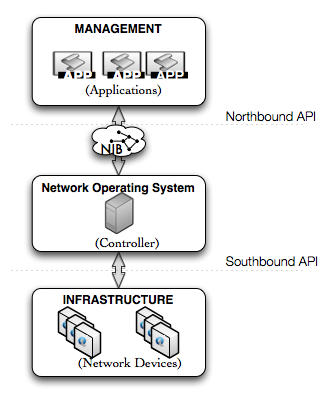
\includegraphics[scale=0.5]{pic/sdn-stack.png}
  \caption[SDN Architecture]{\textbf{SDN Architecture}: is composed by three
    layers: in \textbf{Management} resides the application
    logic that governs the overall network behavior; The
    \textbf{Network Operating System} (NOS)  allows the integration
    of  Management applications and exposes an interface for the
    manipulation of the network (northbound API). It also exposes the Network
    Information Based (NIB); Finally the network is
    represented in the \textbf{Infrastructure} layer. The devices must
  implement an interface allowing configuration (southbound API)}
  \label{fig:sdn-stack}
\end{figure}

\begin{itemize}
\item[] \textbf{Infrastructure Layer:} In this layer are the network
  devices responsible for packet forwarding. Any device 
  can be used (wireless access point, Ethernet switch, router) as long as it implements 
  a standard configuration interface (e.g., OpenFlow). Throughout the text we refer to all these devices as switches;
\item[] \textbf{Network Operating System (NOS):} Provides a standard
  interface to the upper layer (i.e., the northbound interface) allowing the manipulation of the network
  state such as forwarding tables in the managed devices. The
  configuration of devices is actually done by the NOS by interaction
  with the Infrastructure interface for configuration (i.e., the southbound interface). Additionally, it should provide features
  for the integration of Management layer applications.  Throughout
  the text we use NOS, controller or control plane to refer to this
  layer;
\item[] \textbf{Management:} This is where the network logic operates. In this layer
  resides the definition of network level objectives in the form of
  one or more applications. These applications interact with the NIB
  to consult and modify the network state. 
\end{itemize}

The NOS layer provides the northbound API to the upper layers. Network
applications run in the Management layer and can interact with the
network through this API. The NOS layer is also responsible for
communicating with the network devices through the southbound API. The
usual implementation of this API is the OpenFlow protocol.

Notice that the Network Operating System layer plays the intermediary
role in the stack. This implies that not only it allows that
Management applications alter the network state but  also has to
communicate to the Management layer the events that occur at the
Infrastructure level. Complex controllers such as Onix
\cite{Koponen:2010th} use the NIB as the intermediary in this duplex
communication while  the vast majority of controllers only use the NIB as a
simple datastore. 

There must be reliable connectivity between the Network Operating
System and the Infrastructure. The connectivity may be 
\textbf{in-bound} or \textbf{out-bound}
. In the in-bound case the connectivity takes place over the
network used for data forwarding while in the out-bound case a
different and isolated network is used. Connectivity
between these two layers require manual configuration of the
Infrastructure components. 

\subsubsection{Types of Controllers.} The controller is often
categorized in the literature
``logically centralized'' \cite{Gude:2008jd,Greenberg:2005boa}. This concept is used in distributed systems literature
to refer to a physically distributed system that appears, to
its users,  as a
coherent and  transparently distributed service (i.e., it does not
appears to be distributed). The term is perhaps
not well employed in SDN literature as pointed out in
a blog post, by Martin Casado, a Stanford researcher and Nicira
co-founder \cite{:zr}. We will not maintain
this terminology either. Instead, we define that the control platform is 
either  \textbf{distributed} or 
\textbf{centralized} for the remaining discussion. In the centralized
case a single controller is responsible for all the network
Infrastructure as opposed to the distributed case where several
controllers are used.

Another category  distinction in controller software is based on another text
from Casado and Koponen \cite{Martin-Casado:2011ly}, where
three categories of controllers are discussed: 

\begin{itemize}
\item[] \textbf{Single Purpose Controller:} lack support for general management
  applications. Ethane is an example of this type of controllers; 
\item[] \textbf{Thin Controller:} present a northbound interface that is
  strongly-coupled to the southbound interface. Most controllers fall
  under this category. Usually these controllers are known as OpenFlow controllers given the use of OpenFlow in the southbound interface.  
\item[] \textbf{General Controllers:} offer a general purpose service with loosely
  coupled south and northbound interfaces. Transition from the OpenFlow protocol for
  other protocol may  be completely transparent to the Management layer.
\end{itemize}


\begin{itemize}
\item ``Whenever a switch sees a flow's first packet, because there is no flow entry configured on the switch's flow table to match this flow, the first packet will be forwared to the controller. We call this packet a ``flow request''. The controller runs user defined applications to process a flow request, for example the controller computers a path for this flow and installs flow entries on every switch along the chosen path, so that subsequent packets of this flow can be handled by the switches locally. Finally the flow requet packet itself is sent back to the origin switch'' 


\item This reactive model is not ideally. One could also have a proactive model where network changes are applied to the data store view,  resulting (possibly) in configuration changes to the data plane. But typically requirements for the network view are event driven, for example, the location of hosts with OpenFlow is limited to listening and processing packet-in events for flow requests that did not match a flow in the switch table. Typically the installed flow rules to access a host expired on a time basis and/or usage based. This serves two purposes: first it recycles the switch flow tables such that it does not lead to exhaustion of the switch hardware capabilities, but also allows applications to refresh the devices location which can be essential in mobility scenarios caused by mobiles users, virtual machine migration or others. 
But by reverting this tendency to a proactive model with more device drivers (e.g., snmp or others) to access the servers we can avoid this behaviour and have an proactive model whereby the traffic that reaches the controller can possibly decrease in magnitude. Data center measurements suggest that 

\end{itemize}
\subsubsection{OpenFlow}

From openflow.1.3.spec \cite{openflow-spec}
Timeouts : (specified in flow\_mod messages). 
idle timeout - `` If set and the \texttt{hard\_timeout} is zero the entry must expire after \texttt{idle\_timeout} seconds with no received traffic. ''
hard timout  - ``if set the entry must be expired in the specified number of seconds regardless of whether or not packets are hitting the entry. A value of 0 means that a timeout has not been set''
%``If the idle_timeout is set and the hard_timeout is zero, the entry must expire after idle\_timeout
% seconds with no received traffic. If the idle\_timeout is zero and the hard_timeout is set, the entry
% must expire in hard_timeout seconds regardless of whether or not packets are hitting the entry. If both
% idle_timeout and hard\_timeout are set, the 
% ow entry will timeout after idle_timeout seconds with
% no trafficc, or hard_timeout seconds, whichever comes first. If both idle\_timeout and hard\_timeout are
% zero, the entry is considered permanent and will never time out. It can still be removed with a flow_mod
% message of type OFPFC\_DELETE.''

OpenFlow: flowmod and flow removed FIXME 
Maybe talk a little about the asynchronous problems and lacks of guarantees. 
\begin{table}[ht]
  \centering
  \begin{tabular}[ht]{lll}
    Match Fields &  Instructions & Timeouts \\ \toprule 
    source MAC = 10:20:. \emph{AND}  protocol = ICMP  & port 2,3 & 5,10 ms \\ 
    source IP = 10.0.0.0/24  & port 1 &  0/0 \\
    source IP = 10.0.0.0/24 \emph{AND} protocol = TCP & controller & 0/0 \\ 
    any & controller & 0/0 \\ \bottomrule 
  \end{tabular}
  \caption{Simplified representation of a flow table in OpenFlow switches }
  
\end{table}


\begin{itemize}
\item Not event the first packet must go to the controller
\item Wide array of matching. By default each packet is set to a match any . Bitmask masking if supported by the switch (notice the 10.0.0.0/24). 
\item We use an explicit message, but table misses can also be configured to be forwarded to the controller. 
\item wide range of instructions , including multi processing with the use of different flow tables. For our purposes it suffices to understand that we can control the forwarding process with commands as  forward or drop . In the table we only show example that forward the flow to different ports, including an example that forwards it to two different ports. 
\item Hard timeout and idle timeout

\end{itemize}

\begin{itemize}
\item Controller to switch communication. 
\item ``Interface that connects each OpenFLow switch to a controller .  Through this interface, the controller configures and manages the switch, receives events from the switch , and sends packets out the switch'' 
\item Over TCP 

\item Controller to switch
  \begin{itemize}
  \item Messages that are initiated by the controller and may or may note rquire a response from the switch. 
\item Modify state : manage state on the switch and add, delete and modify flow entries in  the OpenFlow tables. 
  \item Packet-out messages used by the controller to send specific messages out a port. 
  \item Barrier messages to ensure message dependencies have been met or to receive notifications for completed operations. 
  \end{itemize}
\item Asynchronous messages 
  \begin{itemize}
  \item Packet-in transfer the control of a packet to the controller. For all packets forwarded to the controller reserved port using a flow entry or the table-miss flow entry. This message contains at least the headers of the data plane message that causes it. In some cases the entire message is sent. Throughout the text we abuse the language and use  the data plane event to refer the packet-in message received at the controller. For example we might say: the controller receives an \gls{ip} request when in practice it receives a packet-in request triggered by an \gls{ip} request at the switch. 
  \item Flow-removed inform the controller about the removal of a flow entry from a flow table. 
  \end{itemize}

\end{itemize}


Message handling
\begin{itemize}
\item Provides reliable message delivery and processing, but does not automatically provide acknowledgements or ensure ordered message processing;
\item It is built over \gls{tcp} but it can not ensure message ordering because multi connections can be open to enhance parallelism; 
\item Messsages are guaranteed eventual delivery unlesss the channel fail; unless the OpenFlow channel fails entirely, in which case the controller should not assume anything about the switch state (e.g., the switch may have gone into ``fail standalone mode'' ) 
\item Ordering can be ensured through the use of barrier messages. in the absence of barrier messages, switches may arbitrarily reorder messages to maximize performance; hence controllers should not depend on a specific processing order. 
\end{itemize}

\begin{itemize}
\item The OpenFlow channel supports multi controllers connectivity
\item The hand-over between controllers is entirely managed by the controllers themselfes.
\item A controller can operate in one of three modes : 
\item In the master mode it has full access to the switch. The switch ensures that only one controller is responsible for this role.  When a controller change its role to master the previous controller is immediately changed to the slave role. 
\item In the slave role the controller only has read-only access to the switch and by default does not receive switch asynchronous messages (except the port status messages that are triggered by changed in the a particular port status - up or down). If this controller attempts to modify the switch state (e.g., flow  modification message) then the switch will reply with an error message
\item Finally the equal role is identical to the master role , but several controller may have it. 
\item Any controller in any role can specify what kind of switch asynchronous messages are received in the controller and which ones it does not cares about. 
\item There is a master identifier to identify how many times the mastership has changed. It is a monotonically increasing counter. When changing a role, the controller must specify an id in the request that is greater than the currently counter seen at the switch, otherwise the message is discarded

\item The switch must be configured at startup with the ip address of the switch. 
\item In case the switch looses connection to all controllers it can enter the fail secure mode or fail standalone mode. In te first the only change is that packets destined to the controller are dropped. Timeout entries are eventually dropped. In the second the switch behaves as a legacy Ethernet switch or router. 
\item On reconnection the flow entries remain. 

\end{itemize}
\section{Physically Centralized  Controllers}
\glsresetall
\label{sec:background:centralized}


In this section we present an overview of relevant centralized
controllers. Centralized controllers are, by our definition, control
planes that do not show any explicit support in the deployment of a
different controllers processes over onde or more servers. 
\subsection{Existent Controllers}
%TODO - what defines a centralized controller. 
%TODO - pipeline as a common model
%TODO - event based
%TODO - thin. 
\subsubsection{NOX}
\label{sec:nox}


%TODO - move to network operating system 
Network Operating System
%TODO make references to section of network operating system 
\begin{itemize}
\item ``Focused on the network operating systems providing an uniform and centralized programmatic interface to the entire network''
\item ``Analalogous to the read and write access to various resources provided by the computer operating systems, a network operating systems provides the ability to observe and controll a network''
\item ``Does not manages the network itself; it merely provides a programmatic interface . Applications implemented on top of the network operating systems perform the actual management tasks.''
\item This interfaces provides the core of a controller. Applications belong to the management layer whereby decisions that affect the switch state is done. The core just affects the controller state (the network view). 
\item Openflow can be seen as a device driver to be used by the network operating system. 
\end{itemize}

NOX
\begin{itemize}
\item Network view.  Could be distributed with standard replication techniques (unspecified) for resilience; 
\item ``The network view contains switch-level topology; the locations of users, hosts, middleboxes and other network elements; and the services (e.g., HTTP or NFS )  being offered but does not include the current state of network traffic;''
\item According to the authors this choice of observation granularity provides adequate information for many network managements tasks and changes slowly enough that it can be scalably maintained in the network; 
\item The choice of flow limits the control application in kind. It can't easily do deep packet inspect for example as it would hinder scalability too much; 
\item ``In terms of consistency; the only network state that is global (i.e., must be used consistently across the controller processes) is the network view; this consistency requirements arises because applications use data from the network view to make control decisions, and those decisions should be the same no matter to which controller instance the flow has been sent. In constract, since neither packet state nor flow state are part of the network, they can be kept in local storage (i.e., packet state in switches, and flow state in controller instances).'' 
\item The netowrk view is a set of indexed hashtables, with extensions for distributed access with local caching to aid scaling across multiple controller instances. 
\item ``Thus, NOX applications should only write to it when a change is detected in the network, and not for every received packet'' 

\item Reactive. Event based.   Pipeline based 
\item The core controller has applications that maintain a switch and host level topology in the network view. Other applications include: discovery of network services, user and host authentication, network policy enforcement, and detect network scanning. 
\item ``Some events are generated directly by \gls{of} messages such as switch koin, switch leave, packet received, port up/dow, and statistics received'';;
\item set of handlers, registered to execute when a particular event handles. Even handlers are executed in order of their priority.
\item Each handlers decides if the event should go further in the pipeline or not
\item Applications handle events and trigger events also. 
\item ``Each service is coupled with an associated event that can be leveraged by other applications''. 


\item It is very intersting to see that the Nox authors consider that NOX can easily scale since the events affecting the network view are in the order of tens of events per second for networks of thousands of hosts. ``The global data structure, the network view, changes slowly enough that it can be maintained centrally (or for resilience, it can be kept consistently on a small set of replicas) for even very large networks'' 
\end{itemize}


NOX \cite{Gude:2008jd}  was published and publicly released under
GPL in 2008. It was both developed in C++ and Python. NOX enables a standard interface for the integration of  Management applications 
in the controller. These applications control
network objectives and also cooperate to define the current
network view (i.e., the NIB). The view is shared between applications. One of the
contributions of the article was the definition of the Network
Operating System abstraction for the controller service. However, NOX
is a Thin Controller. 

\begin{figure}
  \centering 
  \footnotesize
  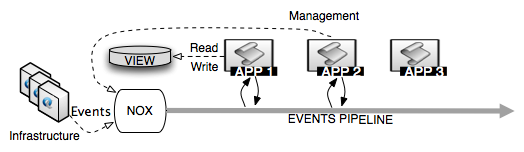
\includegraphics[scale=0.5]{pic/nox-pipeline}
  \caption[NOX pipeline] {\textbf{NOX pipeline} An overview of the NOX
    pipeline used for event processing by the Management applications. NOX
  receives events that have originated either in the Infrastructure of
the Management layer and dispatches them through a pipeline of
applications who have registered for processing these events. 
 As an example: \emph{PACKET\_IN} is a network event while
\emph{USER\_AUTHENTICATED} could be an application event.}
  \label{fig:nox-pipeline}
\end{figure}

NOX is a component framework with primitives for
construction and deconstruction of OpenFlow
based messages. The programming model is event-based. Applications (the components) are registered in a
priority based pipeline with event handlers associated to either
OpenFlow or applications events. This process can be seen in Figure
\ref{fig:nox-pipeline}, which describes the NOX dispatching behavior. Notice
that applications decide if the event should continue to be processed
by the pipeline. NOX  currently ships
with several applications (e.g., forwarding, topology discovery, host
tracking, spanning tree, layer two switch behavior, etc.).

NOX is a centralized controller  but the authors argue that it can easily be distributed for resilience if the shared state (the \emph{view}) is consistently distributed. 
Initially it was a single threaded application not focused on
performance. However, from its publishing date 
several improvements have taken place
\cite{Tootoonchian:2012uia,zen-doc-thesis} that have significantly improved
NOX performance. Under the set of improvements we highlight the
natural evolution to a multi-core aware application
that statically distributes network requests to different threads. 

In the time of writing, NOX is publicly available but has ramified into
two different applications: A C++ based controller available in
Linux and a Python  based controller (POX) available for
several environments \cite{nox}.

\subsubsection{Maestro}
\begin{itemize}
\item ``In general operating systems can be sseen as revolving around two basic purposes: providing applications with a higher level of abstraction so they need not deal with low-level details, and (ii) controlling the interactions between applications. Maestro focuses on the second , ``orchestrating" the contrl decisions made by various management applications''
\end{itemize}

Performance , fairness 
\begin{itemize}
\item Focused in fair service from the controller to the switches requests. while achieving the maximum performance requirements (low request handling and scalability on multi core processors
\item ``We investiage what software design strategies would optimize the eprformacen of a controller machine under the workload characteristics of OpenFlow; assuming the hardware is a commodity computer based on a modern multi-core processor architecture''
\item Otpimizing performacen requires a balancen between fairness, latency, and throughput 
\item The controlelr must be able to run multiple copies of user applications in parallel to scale up throughput on multi-core processors and must do so while maintaining fairness and controlable latency.
\item Users of the system must have the option to write simple single-threaded applications and leave it to the controller to parallelize them. 
\item Found that the round-robin design achieves far superior and near optimal fairness while having excellent scalability, second only to the dynamic partition design. 
\item Also present a workload-adapative request batching algorithm that automatically selects the granularity for batching requests for improved throughput while ensuring request handling latency is well controlled. 
\item NOX and BEacon both statically assign the request from a fixed subset of the network switches to each worker thread. This design maximizes parallelism and is conceptually ideal when requests are uniformly arriving from all switches. 
\item Maestro shows that even under a uniform workload from the swithces, not all worker threads run at exactly the same rate in practice, leading to a performance bias towards some switches. When not uniform, this design suffers from poor fairness and potentially suboptimal throughput due the under-utilization of some worker threads. 
\item Maestro shows that while NOX and Beacon can achieve impressive raw aggregate throughput, as expected such a static batching strategy laeds to unnessarily large request handling latency when the system is under heavy load. 


\item Maestro dynamically creates multiple worker threads, to work on multiple instances of the parallelized application. Furthermore it can stall pending application instances until the update of the shared network state is updated. 
\end{itemize}

\begin{description}
\item[Shared-Queue] A select thread to read the incoming requests from the switches without blocking; Afterwars the requests are put inside a queue shared by all worker threads. One of the workers fetches the requests and leads him through the pipeline until completion;
\item[Maestro-Static-Partition] Adresses the previous design by statically distributing each (or groups of ) switch socket to a different thread. This removes the need for synchronization in the shared queue design; This is the model followed by both NOX and Maestro 
\item[Maestro-Dynamic-Partition] Improves by measuring the switch recent input rates and dynamically arranging the workers-to-switch-sockets binginds. This improves the system since a static partition model does not takes into account that different switches can impose different workloads on the controller 
\item[Round Robin ] Each worker thread is individually running a round-robin service loop among all switch sockets. Each flow request is processed entirely by one of the worker threads, 
\end{description}

\begin{itemize}
\item Found that round robin achieves the most balanced performance for the Controller but stays second best in throughput scalability. The first is dynamic partition but at the cost of increased delay. 
\item Interesting analysis and complete study of the tradeoffs. But it may be that this parallel model is not well adapted to some controller requirements. It is not clear for instance if switches events can be processed out of order. For instances two successive events considering the state of a port are better handled in \emph{First-In-First-Out} (FIFO) sequence). But not even the \gls{of} standard specifies this clearly. 
\item This also does not take into consideration the impact of blocking calls made by the worker threads to remote services that have an impact of latency. 
\end{itemize}

Maestro is the undergoing work of Zeng Cai covered in
\cite{maestro}. It is presented as a Network Operating System focused
in coordination and isolation of the applications  that control the
infrastructure layer. Cai recognizes that Management components do not
operate independently and in isolation. Instead, they operate
concurrently with inter-dependent state (present in the NIB). With this in mind
it aims to exploit parallell computing benefits in the control plane. 

Maestro splits the regular pipeline execution such that it can
be concurrently executed. As seen in Figure \ref{fig:maestro-pipeline} events may
follow different execution paths since singular control components are
not interested in every single event. Thus, Maestro can manage to
execute several applications concurrently. However, in order to
coordinate the control component access to the NIB Maestro opts to
have a more granular network state model. The author argues that it is
common to control components to be  interested only in  subsets of the
NIB. In order to employ concurrent execution Maestro requires that
applications specify  what subsets of the NIB they require as input
and what subsets they modify as output. 

Maestro employs
coordination of the  execution of the applications with performance in
mind. As an example based on Figure \ref{fig:maestro-pipeline} if the routing table
(subset of the NIB) is updated while the RouteFlow application is running, then
Maestro makes sure that the application will use the old version of
the RoutingTable.

\begin{figure}
  \centering 
  \footnotesize
  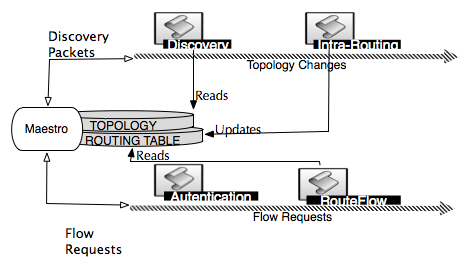
\includegraphics[scale=0.5]{pic/maestro-pipeline.png}
  \caption[Maestro pipeline]{\textbf{Maestro pipeline} Maestro split the pipeline execution
  into several concurrent pipelines based on the events applications
  process and the state they access or modify. In the figure we can
  see two execution paths: \textbf{Topology Changes} processes the
  events triggered by changes in the Infrastructure and \textbf{Flow
    Requests} processes new flow events.}
  \label{fig:maestro-pipeline}
\end{figure}


The fundamental objective of Maestro is to maximize scalability in a
centralized control plane. To do so it attempts to exploit
parallelization in the controller server. Three major design goals
shape Maestro: fair distribution of work across cores; minimal
overhead introduced by cross-core and cache synchronization and;
minimal memory consumption. In addition, it also
exploits throughput optimization through batching. The results
published show that Maestro linearly scales the throughput with the number of cores
available on the controller. 


Currently Maestro is available under the LGPL 2.1 licence. It ships
with usual switching  and routing capabilities \cite{maestro}.


\subsubsection{Beacon}
\label{sec:beacon}
Beacon is an open source controller built in Java, by David Erickson during his academic studies in Stanford University. 
He is, to our knowledge, the only official maintainer of the
application. 

Beacon is also a Thin Controller with  an event-based programming model. Applications register for
specific type of events and process these  in the order
configured by the user. Any application processing an event chooses to forward the
event further in the pipeline or terminate its execution. It is also
multi-threaded, binding switches to particular threads. Applications receive data from all threads.

Applications in Beacon are implemented as \emph{bundles}. A bundle is the
unit of abstraction in the OSGI \cite{osgi} framework - a component and service
platform for the Java programming language with dynamic capabilities -
allowing features such as \emph{hot-swapping} (i.e., deploy, start and
stop modules in run time). 
Beacon provides a central service (the registry) for registration of bundles as
services. Each bundle implements a service, exports it to the registry and
other bundles may consume it. Applications events in Beacon take place
through the service abstraction: bundles may register in other bundles as
listeners to be notified when for specific events take place. 
%TODO - reescrever essa ultima frase. 

Beacon does not provide any NIB service. The network state is
decentralized and encapsulated in the bundle abstraction. There are
no persistance  mechanisms also. 

At the time of writing the applications available are the following: 
 learning switch, hub, device manager , topology, layer 2
shortest path routing, arp  proxy, dhcp proxy. 

%\cite{Controllers: Beacon with David Erickson. Open Network Summit
%  http://www.youtube.com/watch?v=tZ3G_FDuMjg}

\subsubsection{Floodlight}
Floodlight is an open source Apache licensed controller. It was
initially forked from Beacon. It  is developed and maintained by an open community of developers that is mainly composed of Big Switch\footnote{A SDN vendor with a commercial
distributed controller named Big Controller \cite{:vn}.} employers. It is written in Java, but applications can either be
implemented in Java, Jython or through the REST service
available in the NOS (with limited functionality). Floodlight is also a Thin Controller. 

Floodlight follows the common event driven
programming model of most  controllers. Although Floodlight was originally
forked from Beacon, the OSGI support was taken for performance and
deployment reasons. The overall functionality is based on modules
(i.e., applications) that implement services that can be consumed by
other modules. It is similar to Beacon in this regard, however the
module/service functionality is directly provided by Floodlight
instead of delegated to a third-party framework as OSGI. 

Floodlight is also multi-threaded. It accomplishes this through an
asynchronous event based multithreaded library named Netty \cite{netty} that manages Input/Ouput communication with the managed
switches. 

Currently the applications available are: topology manager,  link
discovery, forwarding, device manager, storage, firewall and
static flow pusher.  

\subsection{Controller Choice}
In this section we present an overview of relevant centralized
controllers. Centralized controllers are, by our definition, control
planes that do not show any explicit support in the deployment of a
different controllers processes over onde or more servers. 

%TODO - what defines a centralized controller. 
%TODO - pipeline as a common model
%TODO - event based
%TODO - thin. 
\subsection{NOX}
\label{sec:nox}
NOX \cite{Gude:2008jd}  was published and publicly released under
GPL in 2008. It was both developed in C++ and Python. NOX enables a standard interface for the integration of  Management applications 
in the controller. These applications control
network objectives and also cooperate to define the current
network view (i.e., the NIB). The view is shared between applications. One of the
contributions of the article was the definition of the Network
Operating System abstraction for the controller service. However, NOX
is a Thin Controller. 

\begin{figure}
  \centering 
  \footnotesize
  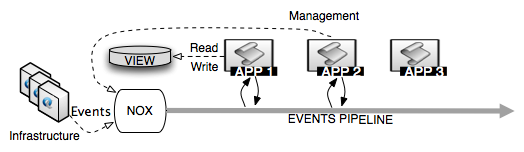
\includegraphics[scale=0.5]{pic/nox-pipeline}
  \caption[NOX pipeline] {\textbf{NOX pipeline} An overview of the NOX
    pipeline used for event processing by the Management applications. NOX
  receives events that have originated either in the Infrastructure of
the Management layer and dispatches them through a pipeline of
applications who have registered for processing these events. 
 As an example: \emph{PACKET\_IN} is a network event while
\emph{USER\_AUTHENTICATED} could be an application event.}
  \label{fig:nox-pipeline}
\end{figure}

NOX is a component framework with primitives for
construction and deconstruction of OpenFlow
based messages. The programming model is event-based. Applications (the components) are registered in a
priority based pipeline with event handlers associated to either
OpenFlow or applications events. This process can be seen in Figure
\ref{fig:nox-pipeline}, which describes the NOX dispatching behavior. Notice
that applications decide if the event should continue to be processed
by the pipeline. NOX  currently ships
with several applications (e.g., forwarding, topology discovery, host
tracking, spanning tree, layer two switch behavior, etc.).

NOX is a centralized controller  but the authors argue that it can easily be distributed for resilience if the shared state (the \emph{view}) is consistently distributed. 
Initially it was a single threaded application not focused on
performance. However, from its publishing date 
several improvements have taken place
\cite{Tootoonchian:2012uia,zen-doc-thesis} that have significantly improved
NOX performance. Under the set of improvements we highlight the
natural evolution to a multi-core aware application
that statically distributes network requests to different threads. 

In the time of writing, NOX is publicly available but has ramified into
two different applications: A C++ based controller available in
Linux and a Python  based controller (POX) available for
several environments \cite{nox}.

\subsection{Maestro}

Maestro is the undergoing work of Zeng Cai covered in
\cite{maestro}. It is presented as a Network Operating System focused
in coordination and isolation of the applications  that control the
infrastructure layer. Cai recognizes that Management components do not
operate independently and in isolation. Instead, they operate
concurrently with inter-dependent state (present in the NIB). With this in mind
it aims to exploit parallell computing benefits in the control plane. 

Maestro splits the regular pipeline execution such that it can
be concurrently executed. As seen in Figure \ref{fig:maestro-pipeline} events may
follow different execution paths since singular control components are
not interested in every single event. Thus, Maestro can manage to
execute several applications concurrently. However, in order to
coordinate the control component access to the NIB Maestro opts to
have a more granular network state model. The author argues that it is
common to control components to be  interested only in  subsets of the
NIB. In order to employ concurrent execution Maestro requires that
applications specify  what subsets of the NIB they require as input
and what subsets they modify as output. 

Maestro employs
coordination of the  execution of the applications with performance in
mind. As an example based on Figure \ref{fig:maestro-pipeline} if the routing table
(subset of the NIB) is updated while the RouteFlow application is running, then
Maestro makes sure that the application will use the old version of
the RoutingTable.

\begin{figure}
  \centering 
  \footnotesize
  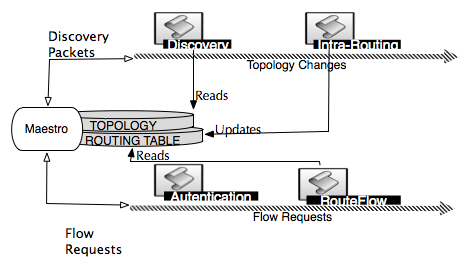
\includegraphics[scale=0.5]{pic/maestro-pipeline.png}
  \caption[Maestro pipeline]{\textbf{Maestro pipeline} Maestro split the pipeline execution
  into several concurrent pipelines based on the events applications
  process and the state they access or modify. In the figure we can
  see two execution paths: \textbf{Topology Changes} processes the
  events triggered by changes in the Infrastructure and \textbf{Flow
    Requests} processes new flow events.}
  \label{fig:maestro-pipeline}
\end{figure}


The fundamental objective of Maestro is to maximize scalability in a
centralized control plane. To do so it attempts to exploit
parallelization in the controller server. Three major design goals
shape Maestro: fair distribution of work across cores; minimal
overhead introduced by cross-core and cache synchronization and;
minimal memory consumption. In addition, it also
exploits throughput optimization through batching. The results
published show that Maestro linearly scales the throughput with the number of cores
available on the controller. 


Currently Maestro is available under the LGPL 2.1 licence. It ships
with usual switching  and routing capabilities \cite{maestro}.

\subsection{Beacon}
\label{sec:beacon}
Beacon is an open source controller built in Java, by David Erickson during his academic studies in Stanford University. 
He is, to our knowledge, the only official maintainer of the
application. 

Beacon is also a Thin Controller with  an event-based programming model. Applications register for
specific type of events and process these  in the order
configured by the user. Any application processing an event chooses to forward the
event further in the pipeline or terminate its execution. It is also
multi-threaded, binding switches to particular threads. Applications receive data from all threads.

Applications in Beacon are implemented as \emph{bundles}. A bundle is the
unit of abstraction in the OSGI \cite{osgi} framework - a component and service
platform for the Java programming language with dynamic capabilities -
allowing features such as \emph{hot-swapping} (i.e., deploy, start and
stop modules in run time). 
Beacon provides a central service (the registry) for registration of bundles as
services. Each bundle implements a service, exports it to the registry and
other bundles may consume it. Applications events in Beacon take place
through the service abstraction: bundles may register in other bundles as
listeners to be notified when for specific events take place. 
%TODO - reescrever essa ultima frase. 

Beacon does not provide any NIB service. The network state is
decentralized and encapsulated in the bundle abstraction. There are
no persistance  mechanisms also. 

At the time of writing the applications available are the following: 
 learning switch, hub, device manager , topology, layer 2
shortest path routing, arp  proxy, dhcp proxy. 

%\cite{Controllers: Beacon with David Erickson. Open Network Summit
%  http://www.youtube.com/watch?v=tZ3G_FDuMjg}

\subsection{Floodlight}
Floodlight is an open source Apache licensed controller. It was
initially forked from Beacon. It  is developed and maintained by an open community of developers that is mainly composed of Big Switch\footnote{A SDN vendor with a commercial
distributed controller named Big Controller \cite{:vn}.} employers. It is written in Java, but applications can either be
implemented in Java, Jython or through the REST service
available in the NOS (with limited functionality). Floodlight is also a Thin Controller. 

Floodlight follows the common event driven
programming model of most  controllers. Although Floodlight was originally
forked from Beacon, the OSGI support was taken for performance and
deployment reasons. The overall functionality is based on modules
(i.e., applications) that implement services that can be consumed by
other modules. It is similar to Beacon in this regard, however the
module/service functionality is directly provided by Floodlight
instead of delegated to a third-party framework as OSGI. 

Floodlight is also multi-threaded. It accomplishes this through an
asynchronous event based multithreaded library named Netty \cite{netty} that manages Input/Ouput communication with the managed
switches. 

Currently the applications available are: topology manager,  link
discovery, forwarding, device manager, storage, firewall and
static flow pusher.  


\section{Distributed Controllers}
\glsresetall
\label{sec:relatedWork:distributed}

In this section we provide an overview of Distributed Controllers
existent in the literature. By our definition an distributed
controllers provides explicit support to the deployment of several
controller processes over one or more servers. 

\subsection{HyperFlow}
Motivated by the lack of scalability in centralized controllers, HyperFlow \cite{Tootoonchian:2010vy} 
was created as a distributed controller. The 
authors aim was to provide scalability without sacrificing
the simplicity of management applications  in  centralized controllers. It
is built as a \emph{C++} application on top of the NOX 
controller \cite{Gude:2008jd} requiring minor modifications to the
controller core and is not publicly available. 
\begin{itemize}
\item Passively syncrhonizing network-wide views. HyperFlow localizes decision making to individual controllers, thus minimizing the control plane response time to data plane request. 
\item All controllers share the same eventually consistent view. But no conflicts should arise if the applications respect the rules. 
\item HyperFlow has the benefit of requiring only minor modifications to existing control applications 
\item The author point out that controlelrs benefit from having the state locally since request can be served locally. 
\item Proactively pushes state to other controllers. 
\item Each controller runs as if they are running the entire network. The HyperFlow application captures commands to switches and responses  and redirects them to the appropriate controllers. 
\item CRITIC: Under failure it has to replay all events. This can be time consuming and events grow indefinitely. Under this time the controller can not serve requests. If instead this recovery mechanism is isolated from the controllers then a recovered controller (or other in its place) can start processing network events almost immediately. 
\end{itemize}


\subsubsection{Architecture.} HyperFlow is composed of two main components: the controller application
and an event propagation system. The overall architecture can be seen
in figure \ref{fig:hyperflow-design}. The controller component is
an application built on top of NOX \cite{Gude:2008jd} which implements an event logger
responsible for subscribing to OpenFlow events and a command proxy
capable of sending OpenFlow commands to  network devices. In essence
HyperFlow interposes  between NOX and
Management applications. The event
propagation system allows  communication between HyperFlow
instances and  is built over a distributed filesystem. Communication
is done through channels implemented as files. There are three types of channels: the
control channel where controllers advertise themselves; the data
channel where general interest events are published by every
controller;  and finally the individual controller channel for OpenFlow
commands relevant to the controller who owns the channel. The
communication system is based on the well known \emph{Publish/Subscribe}
model  whereby one defines publishers as senders of
messages and subscribers as the receivers. Publishers do not send
messages directly  to receivers.  Instead,
messages are published in a medium (in this case the channels) and
interested receivers subscribe to publishers through some form of
subscription logic (e.g., channel, topics, etc.). The Publish/Subscribe
model allows the decoupling of both space and time in the
communication between publishers and subscribers. 
HyperFlow leverages on an existing Publish/Subscribe system that provides: 
persistent storage of the events published; \emph{FIFO}
(First-In-First-Out)  ordered delivery of
the messages published by the same controller; and resilience against
network partitioning.

\begin{figure}
  \centering 
  \footnotesize
  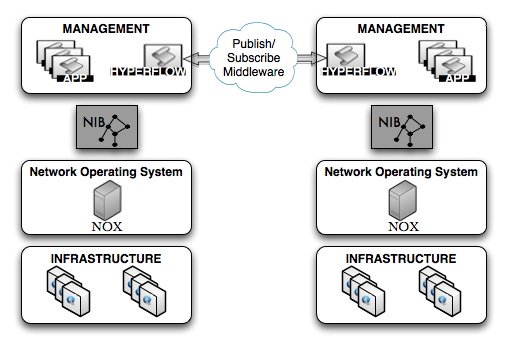
\includegraphics[scale=0.5]{pic/hyperflow-design.png}
  \caption[HyperFlow architecture]{\textbf{HyperFlow architecture} is  similar to
    NOX  with the addition of an Publish/Subscribe middleware
    used between the HyperFlow Management application. The
    Publish/Subscribe system is used for all communication between controllers.}
  \label{fig:hyperflow-design}
\end{figure}


\subsubsection{State Distribution.} State distribution in HyperFlow is accomplished through the
Publish/Subscribe event propagation system. The NIB  is
replicated in all instances and HyperFlow distributes the events
that cause changes to it. This is done through event publishing in the shared
data channel. Every controller subscribes to the
data channel and replays the events received on it, thus changing its
NIB in a similar way.  The view  is maintained by the Management applications
residing in the controller and outside the domain of
HyperFlow (as in NOX). HyperFlow is, in concept,  identical to a \gls{smr} system with the controllers as replicas. State changing events are distributed to all replicas, that execute them to converge to the same state of others. 
But HyperFlow does not guarantee strong
consistency as events are not totally ordered  between controllers. 
Notice that even with FIFO based channels some controller $c$ might receive event $e_i$ followed by event
$e_j$ sent from controllers $i$ and $j$, while a controller $c'$
perceives $e_j$ followed by $e_i$. It is possible that such occurrence
leads controllers to divergent states. The article explicitly adverts
that Management applications should not rely in event ordering "except
those targeting the same entity (e.g., the same switch or link)'' as
those guarantee FIFO ordering. 

Additionally, Hyperflow  also addresses incorrectness problems caused by
transient inconsistency across controllers  by defining an
\emph{authoritative}  controller for each flow. This controller is
responsible for orchestrating changes in the network regarding some
flow. As an example, to avoid loop-free forwarding \emph{authoritative}
controllers are solely  responsible for setting the flow paths across the forwarding
plane for some specific flow. For this, applications must relay
requests for some flow to its \emph{authoritative} controller. 

\subsubsection{Scalability.} HyperFlow addresses scalability of the control plane by minimizing the
number of events that an instance replicates to others. Thus it is
focused on the scalability of the CPU and does not address state
scalability since the NIB is fully replicated in every controller. 

To minimize the number of events  processed by
instances, HyperFlow filters the dissemination of events. To this end
it requires that applications tag locally generated events that affect
the NIB. Only these events are worth distributing as others are redundant. 

Local events are generated either by the Management or
Infrastructure layers but Management applications trigger events as a
response to the processing of other events (i.e., there is a causality
relationship between events). Thus, HyperFlow
minimizes distribution of events even further and if, for example,
some event $e$ is triggered due to the processing event $i$, it 
distributes only event $i$. To this end, Management applications
triggering events have to, both flag the event if it affects the NIB state
but also to associate the event that caused it. As one single event
can cause several application events to be triggered this can reduce
the volume of traffic and processing of redundant events.

\subsubsection{Programming Model.} Applications running on HyperFlow act as they control the entire
network. Behind the scenes  HyperFlow redirects requests to the
network equipment  either to the \emph{authoritative} controller or to the
controller managing the equipment which the request addresses. The choice depends on the type of
the request. HyperFlow also routes back  responses to the controller
responsible for  the request. Also, as previously said, every state
changing event is seen by every controller. So in the end the NIB of
the network contains updated information from every  equipment present
in the network.

The programming model itself is identical to NOX  (event driven,
pipeline based) thus
maintains its simplicity. Some overhead complexity is added as
HyperFlow requires the applications to tag  state changing events and
identify parent events as explained above. 

\subsection{Onix}
Onix \cite{Koponen:2010th}  was build upon the NOX legacy and
provides two major contributions: it is the first general controller
published in the literature, and also the first to provide strong consistency.  Onix 
provides an improved Network Operating System interface on 
which the northbound API does not reflect the southbound
API. Management applications are programmed against a network
graph of Typed Entities very similar to the Object Oriented paradigm
and are not aware of the southbound characteristics (e.g., the use of Openflow). The graph is implemented in 
the \emph{Network Information Base}
(NIB) and can be distributed across a  cluster of  Onix
controllers. Applications have the choice to specify consistency and
durability requirements  per network entity  present in the NIB. 
Onix was the result of a joint effort between Google, NEC, Nicira,
ISCI and Berkely, and (at least)  both Google and Ericson have
developed their controllers based on from Onix \cite{The-Valley-of-the-Nerd.:fk}. At the time of
writing Onix is not publicly available. 

\subsubsection{Architecture.} Onix architecture is presented in figure \ref{fig:onix-design}. Only
one application resides on the 
Management layer and may communicate with other applications in other
controllers instances for coordination. The NIB is the
only element in Onix northbound interface. The Management layer
directly modifies the NIB and subscribes to changes on it. The Infrastructure layer
indirectly modifies the NIB (trough the NOS layer). The NOS has to
guarantee that changes in the Infrastructure are reflected in the NIB
and vice versa. For this, it translates network events into changes in
the NIB and changes in the NIB to changes in the Infrastructure configuration. Onix
supports This process is represented in figure
\ref{fig:onix-process}.  OpenFlow but it could transparently move to another
southbound API. 

Each Onix instance  independently manages a subset of the
Infrastructure. However the NIB  exposes all the network for each
instance. As such, each time a local Onix instance alters the NIB these
changes are reflected in all other instances. Thus, the NIB is also
the distribution mechanism of the Onix controller. The  distribution
itself is done by the datastores that back up  the NIB state (seen
in figure \ref{fig:onix-design}).

\begin{figure}
  \centering 
  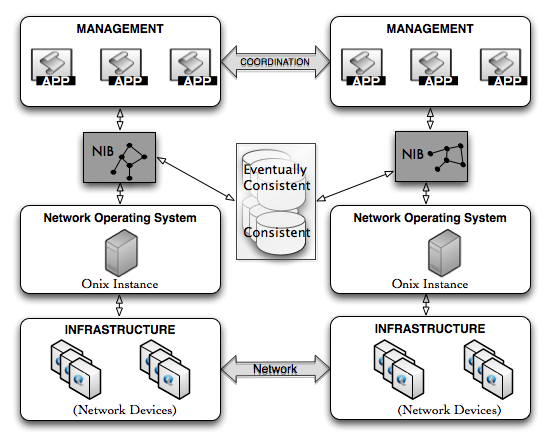
\includegraphics[scale=0.5]{pic/onix-design.png}
  \caption[Onix architecture] {\textbf{Onix achitecture.} In Onix the NIB is the
    solely entity used as the northbound api and Managements program
    directly against it. The NIB is supported by
    two replicated datastores accessible across Onix instances.  The
    Management layer communicates across instances for coordination.}
  \label{fig:onix-design}
\end{figure}

\begin{figure}
  \centering 
  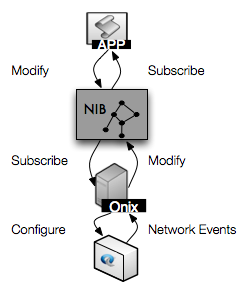
\includegraphics[scale=0.5]{pic/onix-process.png}
  \caption[Onix configuration process]{\textbf{Onix configuration
      process}. The interactions between layers of the Onix
    instance stack. In the figure we can observe the process of
    configuration on the left side, and the process of detecting
    changes in the Infrastructure on the right side.\footnote{The Infrastructure should be only one.}} 
  \label{fig:onix-process}
\end{figure}

\subsubsection{State Distribution.} Onix defines a flexible distribution model for the NIB 
whereby  it offers the application
designer the choice of consistency guarantees. Two
replicated datastores are present, covering  strong 
and  eventually consistency. Strong consistency data is
provided through a transactional persistent database backed up by a replicated
state machine. This datastore is
favored for data with low-frequency changes  as its performance limitations are
significant. The eventually consistent datastore consists in 
an one hop memory based DHT  (as Dynamo 
\cite{DeCandia:2007cn}) favored for  volatile data with high update
rates. 

The NIB reflects the state of both datastores. Both the integration of
datastores and the inconsistency  characteristics of the DHT can lead the
NIB to an inconsistent state where reads performed in some entity may
return more than one result. Thus Onix provides primitives
for the integration of inconsistency resolution logic as well as 
direct integration of a distributed
coordination framework (see  ZooKeeper \cite{Hunt:2010ux}) in the
northbound interface. 

\subsubsection{Scalability.} Onix is intended for large scale Infrastructure where scalability is
fundamental. In each Onix instance the NIB
size reflecting the network state could lead to memory
exhaustion   and the processing of both network events and
subscriptions 
to changes in  the NIB can lead to CPU exhaustion.

In order to introduce scalability and avoid exhaustion, partition and
aggregation based techniques can be configured in the Management
layer. Partition avoids full replication of both data  and workload
such that additional instances do not only replicate overall work but
also relief it. As for aggregation it can, for example, allow network entities to be
aggregated and exposed for other Onix instances as only one.

In practice partition in Onix is present in the division of the
Infrastructure across different Onix instances. 
This way
instances process fewer events. Additionally the Management logic can
configure Onix instances to keep only subsets of the NIB in memory and
up to date. For aggregation, an Onix instance can be configured to
expose a subset of the NIB as an aggregated element. 

\subsubsection{Programming Model.} Applications are built against the NIB graph data structure that is
composed of \emph{Typed Entities} supporting the Object
Oriented paradigm (i.e., encapsulation of data, functions over
entities, hierarchy, etc.). Onix supports extensible representations of
network entities. The
API provides essential functions to search, inspect, create, destroy and
modify entities present in the NIB. It is also possible to register
notifications for creation, removal and updates of data
entities. When network events of other Onix instances update the
datastores those changes must be reflected on the local NIB and the
application must be notified through a callback function. 
All operations are asynchronous, with
eventual delivery and no ordering or latency guarantees given
therefore a \emph{barrier} synchronization primitive is available
allowing the application to wait as
updates are translated and applied in the network devices and/or other
controllers. 

Finally it is worth mentioning that Onix employs coarse-grained
locking mechanisms over the NIB. Applications are given the guarantee
that no other local thread concurrently updates the NIB. 

\subsection{Kandoo}
Kandoo \cite{Yeganeh:2012jm} is an hierarchical controller for
scalable infrastructures. The main
contribution comes from the deployment of isolated controllers near
the switches that shield a parent  controller from processing all
events originating at the network. It is implemented in a mixture of
C, C++ and Python and is not publicly available. 

\subsubsection{Architecture.} In Kandoo --- see Figure  \ref{fig:kandoo-design} --- the controller is split in two levels: in the top level (Network Operating System layer) we
have the root controller responsible for normal operation. In the
bottom (at the Infrastructure layer) we have local controllers that are (ideally)  closer to the
managed switches. This two level design allows  shielding the
controller from frequent events triggered by 
the network devices. Notice that  the entire SDN
stack is replicated in the Infrastructure with the exception of the
NIB since the bottom Management layer should not require direct access to the NIB services. If necessary access to NIB
must be directed to the root controller.

\begin{figure}
  \centering 
  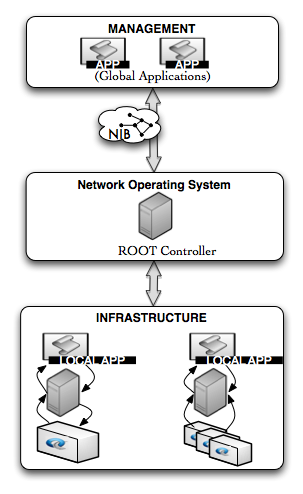
\includegraphics[scale=0.5]{pic/kandoo-design.png}
  \caption[Kandoo design] {\textbf{Kandoo design.} Kandoo decomposes the usual controller
    design into two layers. For this, it brings both controllers and
    applications closer to the Infrastructure. The controllers
    residing in the Infrastructure layer are responsible for
    processing frequent events that do not require access to the
    network state present at the NIB.} 
  \label{fig:kandoo-design}
\end{figure}

This design is motivated by the ideia of bringing control
functionality towards the datapath. As such, \emph{Local Apps} should
require no network wide state and the bottom controllers should stay
close to switches. The deployment of the bottom control plane can
even happen directly at the switches if they support this
functionality (e.g., software switches). 

The remaining design of the controller is not well specified in the
paper. However, other architectures can complement the Kandoo architecture.
The authors stress that even distributing the root
control plane through Onix or HyperFlow is orthogonal to the remaining design.

\subsubsection{Scalability.} In Kandoo scalability is supported by the introduction of the two
level hierarchy. The bottom control plane  shields the root
control from processing of events. As the bottom plane does not
requires access to the NIB it remains simple and
efficient. Additionally, as it is closer to the data plane latency
penalties are lower. However the effectiveness of this
scalability mechanism depends on the Management functionality. For
effective shielding one requires Management applications capable of
operating without access to the network state. The article does not
specifies how practical or significant are this class of
applications beyond exemplifying local policy enforcement  and the
Link Layer Discovery Protocol. 

\subsubsection{Programming Model.} In Kandoo the NOS layer is responsible for the deployment of local
applications in the bottom control plane. The application model only
requires that the applications deployed at the NOS have a flag
that sets its scope (i.e., local or non-local). All the remaining work
is left for the root controller. 

% \subsection{Comparison to Blah, Critic}
% This section is only a scratch for future work orientation. It is
% intended as a comparison to the use of the NIB we are going to build
% and also to criticize the limitations and problems of both HyperFlow
% and Onix. 
% \begin{description}
% \item[TODO] make it clear that HyperFlow replicates controllers. 
% \item[Scalability in Onix] It doesn't exist in the published work (By
%   now it should exist off course). There is quite a bit of blah in the
%   paper about techniques and such but in reality all is left for the
%   application layer to implement relying (again!) on distributed
%   coordination and locking mechanisms; 
% \item[Strong consistency in Onix] Not 100 \% sure about this: it does
%   not exist in practice. If an application mixtures Strong consistency
%   nodes with eventually consistent  links (i.e., (Object A is strong consistent and
%   contains B eventual consistent) it must be prepared to deal
%   with inconsistent resolution upon dealing with the node. The paper
%   suggests this. It is
%   overly complicated in the application logic. 100 \% strong
%   consistency simplifies a lot the application development. 
% \item[Typed entities, Nib Abstraction in Onix] Really cool. higher
%   level of abstraction, another level of indirection. Typed entities
%   combined with the NIB is eternal code loosely coupled to management
%   protocols used in the management of network equipment. Casado
%   defends in a network post
%   [http://networkheresy.com/2011/08/09/what-might-an-sdn-controller-api-look-like-and-should-we-standardize-it/]
%   that it is a general loosely coupled layer, independent of the state
%   distribution mechanism. I disagree, at least in the published
%   work. The state distribution is ``à vista'' in the application layer
%   (define consistency per entity, conflict resolution). It is not
%   fully transparent and consequently not loosely coupled. 

% \item[HyperFlow concept] Kind of reminds a distributed state machine
%   at application level (replay all relevant controller events -i.e.,
%   state changing events) but lacks ordering requirements. 

% \item[HyperFlow] favors availability over consistency. O nosso não
%   fará isso. 
% \item[HyperFlow] sucks. guarantees a bounded window of inconsistency
%   if the network changes trigger less than around 1000 events per
%   seconds. 
% \item[Onix] allows both. The Management deciding. Sacrificing
%   transparency, simplicity. Also, it sucks. 

% \item[Resumo] Hyerflow distribui os eventos o que e estupido porque há
%   muito mais eventos que alteracoes na NIB. Então ele distribui só os
%   eventos que mudam a NIB. O Onix oferece os dois tipos de coerencia
%   mas complica a programacao porque Entities que combinam dois tipos de
%   coerencia podem sempre retornar dois resultados. O Kandoo mete
%   hierarquia ao barulho para minimizar o numero de eventos. 


% \end{description}

\section{Consistent Data Stores}
\glsresetall
\label{sec:relatedWork:consistentDataStore}
%explain 2f+1. 
%Section data stores do artigo. 
The key idea of our controller architecture is to make the controller instances coordinate their actions through a dependable data store in which all relevant state of the network and of its control applications is maintained in a consistent way.
This data store is implemented with a set of servers (replicas) to avoid any single point of failure, without impairing consistency.
One of the most popular techniques for implementing such replicated data store is state machine replication (SMR)~\cite{Sch90,Lam98}.
In this section we review the state of the art on replicated data stores and describe some reasons why, contrary to common belief, they can be a valid option for supporting a distributed controller architecture.

Practical crash fault-tolerant replicated state machines are usually based on the Paxos agreement algorithm for ensuring that all updates to the data store are applied in the same order in all replicas (thus ensuring consistency)~\cite{Lam98}.
Since the original Paxos describes only an algorithmic framework for maintaining synchronized replicas with minimal assumptions, we instead describe the Viewstamped Replication (VR) protocol, a similar (but more concrete) state machine replication algorithm introduced at the same time~\cite{reitblatt2012abstractions}.
Fig. \ref{fig:paxos} shows the messages exchanged in Paxos/VR for an update operation: the client sends a message to a primary replica (the leader) that disseminates the update to all other replicas. These replicas write the update to their log and send an ACK to the primary.
In the final step the leader executes the request and sends the reply to the client.
If the primary fails, messages will not be ordered and thus a new primary will be elected to ensure the algorithm makes progress.
When read-only operations are invoked, the leader can answer them without contacting the other replicas.
Strong consistency is ensured due to the fact that all requests are serialized by the leader.

\begin{figure}[!ht]
\centering
\includegraphics[width=0.5\textwidth]{pic/related/vr.pdf}
\caption[Paxos/VR update protocol]{Paxos/VR update protocol.} 
\label{fig:paxos} 
\end{figure}

The Paxos/VR algorithm has served as the foundation for many recent replicated (consistent and fault-tolerant) data stores, from main-memory databases with the purpose of implementing coordination and configuration management (e.g., Apache'  Zookeeper~\cite{Hun10}), to experimental block-based data stores or virtual discs~\cite{Rao11,Bol11,Bes13}, and even to wide-area replication systems, such as Google Spanner~\cite{Corbett:2012uz}.
Besides the synchronization protocol, these systems employ many implementation techniques to efficiently use the network and storage media.

Although not as scalable as a weakly consistent data store, these systems grant the advantages of consistency for a large number of applications, namely those with moderate performance and scalability requirements. To give an idea of the performance of these systems, Table \ref{table:smr-results} shows the reported throughput for read and write operations of several state-of-the-art consistent data stores.

\begin{table}
  \center
    \begin{tabular}{ lccc}
    \hline
    \emph{System} & \emph{Block Size} & \emph{kRead/s} & \emph{kWrite/s} \\ \toprule
    Spanner \cite{Corbett:2012uz} & 4kB & 11 & 4 \\ 
    Spinnaker \cite{Rao11} & 4kB & 45+ & 4 \\  
    SCKV-Store \cite{Bes13} & 4kB & N/R & 4.7 \\ 
    Zookeeper \cite{Hun10} & 1kB & 87 & 21 \\ \bottomrule 
    \end{tabular}
  \caption[Performance of state machine replication systems]{Throughput (in thousands data block reads and writes per second) of consistent and fault-tolerant data stores based on state machine replication (N/R = Not Reported).}
  \label{table:smr-results}
\end{table}

Given the differences in the design and the environments where these measurements were taken, we present these values here only as supporting arguments for the possibility of using consistent data stores for storing the relevant state of SDN control applications.
Depending on the specific application this state may include, for instance, a subset of the Network Information Base (NIB).
Interestingly, these values are of the same order of magnitude of the reported values for \emph{non-consistent} updates in Onix (33k small updates per second considering 3 nodes~\cite{koponen2010}), and much higher than the reported values for their consistent data store (50 updates/second for transactions with a single update).
The Onix paper does not describe how its consistent database is implemented but, as shown by these results, its performance is far from what is being reported in the current literature.


\section{Consistent Data Planes}
\glsresetall
\label{sec:relatedWork:consistentPlane}


Recent work on SDN has explored this need for consistency at different
levels. Programming languages such as Frenetic~\cite{Foster2011} offer
consistency when composing network policies (automatically solving
inconsistencies accross network applications' decisions). Other
related line of work~\cite{reitblatt2012abstractions} proposes
abstractions to guarantee data-plane consistency during network
configuration updates. The aim of these systems is to guarantee
consistency \textit{after} the policy decision is
made. Onix~\cite{Koponen:2010:ODC:1924943.1924968} provides a
different type of consistency: one that is important \emph{before} the
policy decisions are made. Onix provides network state consistency ---
both weak and strong --- between different controller instances. The
datastore we propose is similar in that it offers strong consistency
for network (and application) state between controllers\footnote{By
  strong consistency we mean that all accesses to the datastore are
  seen by all controller instances in the same order
  (sequentially).}. Our main objective is to improve the ``performance
limitation''~\cite{Koponen:2010:ODC:1924943.1924968} of Onix's
transactional persistent database. 


Other works on SDN consistency include the Frenetic programming language~\cite{Foster2011}, Reitblatt et al. work on abstractions for network update~\cite{reitblatt2012abstractions}, and Software Transactional Networking~\cite{Canini:2013:HotSDN:STN}. 
These papers address different consistency issues, however. 
In essence, they target consistent flow rule updates on switches, dealing with overlapping policies and using atomic-like flow rule installation in SDN devices.
In other words, they take care of data-plane consistency \emph{after} the policy decisions are made by the network applications. 
Frenetic offers a high level language and a run-time system that, besides other benefits, ensures that policy rules made by concurrent network applications are not overlapped, thus avoiding network inconsistencies.
In~\cite{reitblatt2012abstractions} the authors propose two abstractions --- per-packet and per-flow consistency --- and mechanisms to guarantee that on a network update a packet (or a flow) is processed by exactly one consistent global network configuration. 
STN extends these works by proposing a transactional solution to provide consistent rule installation in a distributed setting. 
Our work targets consistency at a different level.
Our datastore ensures strong control-plane consistency for network
and/or applications state, which means policy decisions are always
based on a consistent state.


%%% Local Variables: 
%%% mode: latex
%%% TeX-master: "../PEI"
%%% End: 


\LIMPA
\chapter{Distributed Controller}
%\epigraph{Estamos no Mato...  E sem cão!}{Professor de LEI - 3º ano}
\glsresetall


\section{Controller}
The most interesting thing about this design is that each controller instance can have direct control over the window of inconsistency for every application. 
\subsection{Architecture}

\begin{figure}[ht]
  \centering
  \begin{subfigure}[b]{0.4\textwidth}
                \centering
                \includegraphics[width=\textwidth]{pic/heimdall/global-app}
                \caption{General architecture}
        \end{subfigure}%

        \begin{subfigure}[b]{0.7\textwidth}
                \centering
                \includegraphics[width=\textwidth]{pic/heimdall/instance-design}
                \caption{Controller instance architecture}
        \end{subfigure}
\end{figure}



\begin{description}
\item[Global Application] A global app can be a monitoring app, a web based interface to update network policies, etc., Those apps do not fit in the event-driven programming  model of the controller.  As such they do not need to be inside each controller but rather on a global location that has access to a controller instance. Each controller instance has a REST API that exposes network and data store state according to the native apps decisions and configurations;
\item[Native Application] A native app resides in the controller memory and is an event based application that usually reacts to network changes, flow requests and data store changes. These applications can be replicated across each controller instance. Examples are the Topology Manager, Device Manager, Firewall, Load Balancer and Forwarding applications; 
\end{description} 

\noindent\makebox[\textwidth]{\rule{\paperwidth}{0.4pt}}

Controller Core : 

\begin{description}
  \item[Pipeline Manager] Manages the dispatching of  events to the applications. Applications are registered in this Manager to handle specific events. Events can be triggered by the data plane or the applications itself. When an event  occurs the dispatcher calls applications in a predefined order;
  \item[Pooling Manager] Applications register routine timed operations. Ideally this will support efficient pooling to check changes and/or updates in both the data store and data plane (e.g., counters); 
  \item[Data Store Service] Allows the creation and/or location of tables in the data store. Clients use this to create local objects to manipulate data store tables. Also manages the Cache inside the controller; 
  \item[Switch Communication] Communication with switches (e.g., install rules, consult flow tables). Applications will not have the possibility to directly contact the data plane. This module abstracts this into a service that can later be expanded to handle more complex tasks such as conflicting policies, safety checking, table space reduction etc.,; 
  \item[Network Partition] Handles the controller instance reliability protocol (take over other controllers that have failed);
\end{description}



\subsection{Transactional Memory}

This section presents a rude idea to approach the controller pipeline (processing events by different applications) focusing in performance. The problem it tries to solve is the excessive communication with the data store. 
It is inspired by the micro components approach (having code in the data store such as stored procedures in SQL data bases), transactions and transactional memory. The basic idea is to avoid the data store at all cost. When communicating with the data store, join requests from different switches and applications to batch them. That is it. It may not work every time, but it is still possible to resort to the typical approach in isolated cases.\\


The pipeline: 
\begin{itemize}
\item The controller pipeline is where each application is registered to process the event in order. 
\item A pipeline is defined by the event type. For each event there is a  pipeline with different application as stages. 
\item Each pipeline will be run by a single thread  defined by the source of the event (usually a switch). This way there is no need for locks and concurrency control since each event source will have a private state (e.g., cache). The pipeline is lock-free. 
\end{itemize}

Figure \ref{fig:pipeline} shows the general behaviour of the pipeline. 


\begin{figure}[ht]
  \centering
  \includegraphics[width=0.9\textwidth]{./pic/heimdall/pipeline.pdf}
  \caption{Processing events in the pipeline. A single thread pre-fetches everything that is not existent in cache to the data store. Then each app processes the event locally with no data store communication. In the end we commit to the data store the collection of modifications done by every application. If sucessfull we can proceed to installing a flow rule if necessary. }
\label{fig:pipeline}
\end{figure}


\begin{itemize}
\item The first step is to call each application handler that receives the event and  tells which data it needs to fetch to cache . 
\item The data is fetched to cache in a single operation that groups all the requests from all applications. 
\item Then, we proceed with the event processing by calling each application handler. This time applications do not perform any communication with the data store. Everything is done locally. 
\item In the end we attempt to commit every change made by each application in the data store with a single operation. Notice that this commit can fail if the user wishes to only succeed if the data fetched in the cache phase as not been modified in the data store when we are committing. This enables consistency control of stale data (cache based) if desired. 
\item Finally we can build the outcome of processing the event (e.g, install rules in the switches). 
\end{itemize}

Notes : 
\begin{itemize}
\item We may need an excessive amount of micro components to group operations that need to read, process and then read again. Ideally you want two micro components ``per event'' : one to read stuff into cache, and one to write. When the write happens every time you might as well have a single micro component which does everything in the data store; 
\item Some data may already be present in the cache. So we can avoid reading from the data store in the pre-fetch phase;
\item Some events may not need to write anything to the data store;
\item We could consider Pooling for writes (periodically  update the data store). Imagine: you do not care if a device timestamp is updated 10/20 times in a minute. Every 30 seconds is fine.  
\end{itemize}

Figure \ref{fig:pipeline-seq} shows a possible sequence diagram when processing an event in the pipeline. 

\begin{figure}[ht]
  \centering
  \includegraphics[width=\textwidth]{./pic/heimdall/pipeline-seq.pdf}
  \caption{Processing events in the pipeline. }
  \label{fig:pipeline-seq}
\end{figure}


\subsection{Data Store}

\subsubsection{Domains}
\begin{itemize}
\item A data store domain is an instance of the bft-smart system with a given number of replicas;
\item With different domains we can increase the throughput and latency of the system ; 
\item We can shard tables over domains. For example we could have a global domain for all global tables (accessible by different controllers). Local tables could be available in another domain. At the extreme each controller would have its private domain and a global one. 
\end{itemize}

\subsubsection{Data Store Service}

\begin{itemize}
\item Applications only communicate with each other through the data store. 
\item What application is responsible for some data is not relevant
\item The applications known through the data store service if some kind of application (and respective tables is available) 
\end{itemize}


The data store supports different table types shown in Table~\ref{tab:table-types}. The Global and Global to Application tables must be made available to every controller while the Local and Local to Application can be reachable only to a single controller instance. However in case of failures and controller fail-over one must be certain the backup controllers can reach the failed controller tables. Beyond the types shown each table state can be persistent (kept in disk) or not. The former is of the utmost importance for the controller configuration data (e.g., network policy). Notice however that the state is always kept in memory. If the controller state grows beyond the memory size  of a data store replica then the data can be divided across different domains at the expense of more hardware. 

\begin{table}[ht]
  \centering
  \begin{tabular}{ll}
    Name & Accessibility \\ \toprule 
    Global & Every controller and every application   \\ 
    Global to Application & Single application on every controller \\
    Local & Every app in a single controller \\
    Local to Application &  Single application in a single controller \\ \bottomrule 
  \end{tabular}
  \caption{Table types}
  \label{tab:table-types}
\end{table}


\begin{figure}[ht]
  \centering
  \includegraphics[width=\textwidth]{./pic/heimdall/global-to-local.pdf}  
  \caption{Topology tables in the data store. The local topology represents the entire topology seen by a controller. The global topology shows only the minimum spanning tree.}
  \label{fig:topologies}
\end{figure}

Performing aggregation: 

\begin{itemize}
\item Local Tables can have code in the data store; 
\item Under each write in the local table the code checks if something needs to be written to the global table; 
\item For example Figure~\ref{fig:topologies} shows that the local version of a controller topology table shows every link while the global version (available to every controller) only shows a minimum spanning tree of the local topology.  A controller could even choose to hide the entire topology and just keep all its devices as attached to the border switches (that connect to other controllers data plane domains). 
\end{itemize}

The Data Store Service (DSS) as viewed from the user : 
\begin{itemize}
\item Allows the creation of local objects to communicate with the data store. 
\item Manages the creation of the controller cache, and transactional pipeline entities (Cache Manager, Write Manager). 
\item Guarantees that each event thread gets an isolated environment (its own cache and data store channel). This is important to make the pipeline lock free and also to improve concurrency (different data store channels). 
\item Shields the user from the RPC semantics in the communication with the data store. 
\item Provides a static typed interface for the data store. 
\item Expanded in the future with some kind of query language, which is essential to applications. This will enable a more expressive communication with the data store that is able to filter the values obtained. 
\end{itemize}
\
\subsection{Pooling}
\begin{itemize}
\item Typically controllers are reactive. Floodlight applications have a publish/subscribe behaviour to warn other applications of events. An example is the Device Manager which triggers events for devices that have been created, moved or deleted. The Topology Manager does the same thing on every topology change. 
\item We do not want this behaviour. This would require sending information to all controllers (which would not make sense to do trough the data store). 
\item So each application maintains (if she wishes) a pooling task in the pooling manager. 
\item The pooling manager groups tasks by subscriptions and periodicity. 
\item Checking changes is done with version numbers by table, table entry and (possibly) columns. The data store should have the possibility of tracking changes to the tables between versions. This is crucial for efficiently fetching the devices, or links that have been added or removed between versions. 
\item When changes are made, a pipeline is formed for the applications that subscribed to those changes. 
\end{itemize}

\section{Reliability}
A simple ``protocol'' to handle switch fail-over. I still need to think of bad things that can happen when two controllers fight over a switch.
\subsection{Protocol}
\begin{itemize}
\item There is an eventual failure detector built with the data store. If the controller does not has access to the data store it should not control anything in the network (Fig.~\ref{fig:proto-heartbeats}). The data store also keeps the switches under each controller ; 
\item Controllers can suspect the failure of another and attempt to replace it. First they have to set a flag in the data store stating that they are attempting to take over the presumably failed controller (Fig.~\ref{fig:proto-c2-fails}). With this flag other controllers can known that someone is attempting to control the switches and avoid taking over. This also helpfully for the failed controller which can recover and known that there is an active process to take its place. 
\item A controller can then set himself as master of the switch. After this point all switches messages go to the new controller (C1) (Fig.~\ref{fig:proto-c1-as-master}); 
\item Finally the controller sets himself as master of the switch in the data store. (Fig.~\ref{fig:proto-c1-finishes}). 
\end{itemize}


\begin{figure}
  \centering
  \begin{subfigure}[b]{0.5\textwidth}
                \centering
                \includegraphics[scale = 0.4]{./pic/heimdall/proto-1}
                \caption{Heartbeats sent to the data store. }
                \label{fig:proto-heartbeats}
        \end{subfigure}%
        ~
        \begin{subfigure}[b]{0.5\textwidth}
                \centering
                \includegraphics[scale=0.4]{./pic/heimdall/proto-2}
                \caption{C1 finds out that C2 has failed.}
                \label{fig:proto-c2-fails}
        \end{subfigure}

  \begin{subfigure}[b]{0.5\textwidth}
                \centering
                \includegraphics[scale = 0.4]{./pic/heimdall/proto-3}
                \caption{C1 has to set himself as master in S2. }
                \label{fig:proto-c1-as-master}
        \end{subfigure}%
        ~
        \begin{subfigure}[b]{0.5\textwidth}
                \centering
                \includegraphics[scale=0.4]{./pic/heimdall/proto-4}
                \caption{Finally tell the data store he controls S2. }
                \label{fig:proto-c1-finishes}
        \end{subfigure}
\end{figure}

Notes
\begin{itemize}
\item In the case S1 fails while taking over S2, other controllers (if any) will eventually known about this and take over. 
\item This process can also be triggered in the case a switch fails. It is worth doing so because a switch can fail due to network failures who affect the connectivity with his master controller but not with others; 
\item As long as one  controller does not fail and reaches every switch (who also has not failed)  and data store we can handle all kind of network failures.
\item When C2 recovers he can do the same process to take over his switches again. 
\item I think that to be safe (I will try to define safety later) the data store should deny state changing messages from controllers who do not own the switch (which caused the state changes). But I have to think better about this.... 
\end{itemize}

% \linebreak

% \section{Shared Data Store Controller Architecture}
% \glsresetall
% \label{sec:heimdall:architecture}
% %%%%%%%%%%%%%%%%%%%%%%%%%%%%%%%%%%%%%%%%%%%%%%%%%%%%%%%%%%%%%%%%%%%%%%%%%%%%%%%%%%%%%%%%%%%%%%%%%%%%%

% The proposed distributed control architecture is based on a set of controllers acting as clients of the fault-tolerant replicated key-value data store, reading and updating the required state as the control application demands, maintaining thus only soft state locally.
% There are two main concerns around this design: (i) how to avoid the storage being a single point of failure and (ii) how to avoid making the storage a bottleneck for the system.
% In the previous section we showed that state-of-the-art state machine replication can be used to build a data store that solves both these concerns.


% Fig. \ref{fig:architecture} shows the architecture of our shared data store distributed controller.
% The architecture comprises a set of SDN controllers connected to the switches in the network.
% All decisions of the control plane applications running on the distributed controller are based on OpenFlow events triggered by the switches and the consistent network state the controllers share on the data store.
% The fact that we have a consistent data store makes the interaction between controllers as simple as reading and writing on the shared data store: there is no need for code that deals with conflict resolution or the complexities due to possible corner cases arising from weak consistency.

% By design, the SMR-based data store is replicated and fault-tolerant (as in all designs discussed in the previous section), being up and running as long as a majority of replicas is alive~\cite{Lam98}.
% In other words, $2f+1$ replicas are needed to tolerate $f$ simultaneous crashes.
% Thus, besides offering strong consistency, this architecture leads to a completely fault-tolerant control plane.
% Furthermore, in this design the controllers keep only soft state locally, which can be easily reconstructed after a crash.
% The switches tolerate controller crashes using the master-slave configuration introduced in OpenFlow 1.2\,\cite{ONF2011}, which allows each switch to report events to up to $f+1$ controllers (being $f$ an upper bound on the number of faults tolerated), with a single one being master for each particular switch.
% The master is constantly being monitored by the remaining $f$ controllers, which can takeover its role in case of a crash.

% Interestingly, our architecture could also be used in SDN deployments were a distributed controller is not necessary, to implement fault tolerance for centralized controllers.
% In this case the fault-tolerant data store can be used to store the pertinent controller state, making it extremely simple to recover from its crash.
% In this case, the applications deployed on the primary controller manage the network while a set of $f$ backup controllers keep monitoring this primary, just as in the distributed controller design.
% If the primary fails, one of the backups -- say, the one with the highest IP address -- takes the role of primary and uses the data store to continue controlling the network.

% Our distributed controller architecture covers the two most complex fault domains in an SDN, as introduced in~\cite{kim2012}.
% It has the potential to tolerate faults in the controller (if the controller itself or associated machinery fails) by having the state stored in the fault-tolerant data store.
% It can also deal with faults in the control plane (the connection controller-switch) by having each switch connected to several controllers (which is ongoing work).
% The third SDN fault domain --- the data plane --- is orthogonal to this work since it depends on the topology of the network and how control applications react to faults.
% This problem is being addressed in other recent efforts~\cite{kim2012,Reitblatt2013}.

% \begin{figure}
% \centering
% \includegraphics[scale=0.6]{./pic/heimdall/multicontroller.pdf}
% %add desired spacing between images, e. g. ~, \quad, \qquad etc.
% %(or a blank line to force the subfigure onto a new line) 
% \caption[Heimdall Architecture]{The shared data store controller
%   architecture with each switch sending OpenFlow messages to two
%   controllers. The controllers coordinate their actions using a
%   logically centralized data store, implemented as a set of
%   synchronized replicas. }
% \label{fig:architecture} 
% \end{figure}

% \section{Floodlight} 
% \glsresetall
% \label{sec:heimdall:floodlight}
% %%%%%%%%%%%%%%%%%%%%%%%%%%%%%%%%%%%%%%%%%%%%%%%%%%%%%%%%%%%%%%%%%%%%%%%%%%%%%%%%%%%

% \section{Data Store}
% \glsresetall
% \label{sec:heimdall:dataStore}
% %Features  design, etc., 
% \label{sec:heimdall:datastore:bft-smart}
% FIXME : Alysson - será que posso justificar que a data store
% performance nao é importante quando comparada com o middleware? 

% \subsection{Smart}
% we had to change the library used of netty from netty-3.1.1.GA.jar to
% netty-3.2.6.Final.jar because it conflicted with floodlight. We are in
% the dark here. Do not known if this will cause problems... 

% \subsection{Implementation}

% \subsubsection{Map interface} 
% Actually motivated by the LearningSwitch application. The rest interface exposed the learning switch database (hash table ) directly. We implemented a class to Delegate the map interface methods to our KeyValueTable. We don't actually use it inside the applications we modified because we have some preference for static typing (which for arguably legitimate reasons does not appear in the Map interface). Nevertheless we could use it. putAll and containsValue are not implemented. No special reason just lazinesss.  

% LinkedHashMap should be used for maintaining consistent ordering
% across replicas. 
% \pagebreak 
% \section{Data store}
% \label{sec:heimdall:datastore:functionalities}

\subsection{Prototype Implementation}
\textbf{Isto vai ser uma secção a falar do protótipo de base de dados implementado.} 
\begin{figure}[ht]
  \centering
  \includegraphics[scale=0.6]{./pic/heimdall/client-tables-classes.pdf}
  \caption{Class diagram of the client interface to the data store tables.}
\label{fig:design:class-diagram}
\end{figure}

Missing things to talk about: 
\begin{itemize}
\item An hash table and a Key Value table is the same, we use both terms. 
\item Define \gls{rpc} messages as the messages that are sent to the data store to perform an operation. 
\item Define marshalling/unmarshalling as the process to convert an object into a byte representation and vice-versa. 
\end{itemize}

We implemented a  data store prototype that has been iteratively refined to incorporate data store functions required to increase the performance of real world applications (discussed in Chapter~\ref{sec:feasibility:apps}).  
Fig~\ref{fig:design:class-diagram} shows the class diagram for the client side interfaces that allow him to communicate with the  data store.  
\begin{itemize}
\item \emph{ITable} interface introduces the general functionality of a key value table.
\item \emph{IKeyValueTable}  is a normal hash table. You can manipulate the key to value association in different ways. It extends a \emph{ITable}
\item \emph{IColumnTable} is the extension of a \emph{IKeyValueTable} into a bi-dimensional table where two keys access an individual value. 
\item \emph{ICachedKeyValueTable} allows explicit control over the window of inconsistency accepted in cached values for an \emph{IKeyValueTable} 
\item \emph{ICachedColumnTable} does the same for an \emph{IColumnTable} 
\end{itemize}

This is not a lesson in design. The interfaces presented are part of a prototype that we leveraged to capture the behaviour of applications, and perform a requirement study for the data store. Off course that in production code we can use any of the existent off the shelves data stores (either SQL or NoSql) given that they offer the same functionalities that we present in this section. 
\label{sec:heimdall:key-value}

\subsection{Cross References} 
\label{sec:heimdall:cross-references}
A Cross Reference table ($t_{cr}$) contains values that can be used as keys in another table ($t_{d}$). 
Therefore a data store client can use a key valid in  one table ($t_{cr}$) to retrieve a value at  a different table ($t_{d}$) but with the benefit of using a  single data store operation (the \texttt{getCrossReference} method at \emph{IKeyValueTable}). 

Commonly, despite the number of unique attributes that can be used to identify a value, we are limited to using a single one when using an hash table. 
Commonly, an hash table is restricted to a single key to identify a value despite the  number of unique attributes  that can be used to identify it. 
Furthermore, the asymptotical complexity to obtain a value with a particular key is \BigO{1} as opposed to searching for one which, at best, has $\Omega(\log n)$ complexity for $n$ entries (using balanced trees). 

To circumvent those limitations, one can use an additional table that relates a ``secondary'' key of a value to its ``main'' one. 
To clarify, imagine that for the purpose of tracking hosts in a network we consider that a device is uniquely identified by an \gls{ip} or \gls{mac} address. 
Therefore, we could use two tables: one relating \glsplural{ip} to  \glsplural{mac}, and another relating \glsplural{mac} with devices.

This is a reasonable scheme in a local environment (in memory hash table) given that the asymptotical cost to obtain a device with 
a \gls{mac} address or its \gls{ip}  are equal (\BigO{1}). 
However, in a distributed environment, this scheme requires two round trips to the data store just to obtain a single device with a \gls{ip} address (one to fetch the \gls{mac}, and another to fetch the device). 

Seing that this was a common behaviour in the existent Floodlight applications that we modified to use our data store, we developed the Cross Reference functionality which, as shown in chapter~\ref{sec:feasibility:apps}, results in a significant performance improvement. 
With it, the clients are able to create multiple Cross References tables to track values using different uniques attributes. 
As a result, despite the key that a client uses to obtain a value it can always do it with a single operation. 


\subsection {Versioning}
\label{sec:heimdall:versioning}
\begin{figure}[ht]
  \centering
  \begin{subfigure}[b]{0.5\textwidth}
                \centering
                \includegraphics[width=\textwidth]{./pic/heimdall/versioning-0}
                \caption{No Versioning.} 
                \label{fig:heimdall:versioning-0}

        \end{subfigure}
        ~
        \begin{subfigure}[b]{0.5\textwidth}
                \centering
                \includegraphics[width=\textwidth]{./pic/heimdall/versioning-1}
                \caption{Versioning.}
                \label{fig:heimdall:versioning-1}
        \end{subfigure}
  \caption[Concurrent updates]{The concurrent update to the \texttt{visitors} set for a particular site can result in loss of data. In  Fig.~\ref{fig:heimdall:versioning-0} the update from client 1 is forgotten  when replaced by the update from client 3 (last-write-wins).  Conversely in Fig~\ref{fig:heimdall:versioning-1} the use of versioning in the data store prevents client 2 from overwriting the last update.}
\label{fig:heimdall:versioning}
\end{figure}

With Versioning we associate each table entry (i.e., key value pair)  with a monotonically increasing counter --- the version number ---   that is incremented in every mutation operation. 
Doing so, we empower the data store with the capability to detect and prevent conflicting updates that otherwise could result in the loss of data. 

To clarify, imagine an \gls{http}\footnote{The application protocol for distributed, collaborative, hypermedia information systems.} network logger running in a controller that maintains  a Key-Value table  (in the data store) to map each \gls{url}\footnote{A uniform resource locator, also known as web address,  that constitutes a reference to a resource such as a web page or email.} seen to the set of \gls{ip} addresses that have visited it. 
Whenever a hosts visits a site, the controller adds the \gls{ip} address of that host to the site visitors set. 
However, being that  for the data store a set is merely an opaque binary object, the controllers are forced to fetch the set, add an element locally and finally write the new set in the data store. If two controllers do this concurrently, then it is possible to loose values added to the set. 

Fig.~\ref{fig:heimdall:versioning-0} shows how this update algorithm can result in data loss in the context of concurrent updates. 
First, controllers 1 and 2 fetch the same \texttt{visitors} set for a particular site (uniquely identified by the \gls{url}), then they replace it by a new set that includes IP2 and IP3 respectively. 
In this case the lack of concurrency control  results in the loss of the write operation that includes the IP1 visit to the site (visitors={IP2,IP3})  since the  last write (visitors = {IP1, IP3}) overwrites the previous. 

Fig~\ref{fig:heimdall:versioning-1} shows that with Versioning, the write from controller 1 results in an increase of the version number of the visitors set at the data store (to 2) which prevents any update done by controllers unaware of the most recent version of the set. 
Therefore, by the time the second write request (from controller 2) arrives at the data store it can be aborted since  the version number included in the operation is not consistent with the data store. 


Whenever the data store denies a request (as in the example above) the client can only repeat the entire process since that in order to complete its write, it must obtain the current version number which is obtained from reading the value from the data store. 
To be true, it is often the case that the correct behaviour requires reading the value again, since the client write is built over the existent value in the data store. 
Otherwise, the client would have used a ``free'' write operation not subjected to the data store version verdict. 


It is important to realize that the data store has no mechanism to guarantee that a stubborn client will eventually succeed.
Indeed, it is possible that one client  loops indefinitely if another client constantly out-wins him in every write attempt. 
Clients are solely accountable for  guaranteeing  the progress (liveness) of their updates. 
This process is commonly termed of \emph{Optimistic Concurrency Control}. Clients are optimistic in the sense that they hope that no one else updates the value while they perform the entire process (read, modify and write). 

The Java common library provides a concurrent hash table (\emph{ConcurrentHashMap}) with concurrent control primitives  equivalent to the ones we include in our data store \gls{api}. 
However, the control is based on the logical equivalence of values instead of version numbers. 
That is to say, that instead of providing the version number in a conditional write, the client must provide the value that it expects to find in the hash table. 
Then, the hash table implementation can perform a logical test to assert if the client provided value is logically equivalent to the one that it holds. If so, the write is allowed, otherwise it is ``aborted''.  

While adapting existing applications to our \gls{api} that used the Java concurrent hash table, we have chosen to modify them slightly to use the version number mechanism instead of the existent logical equivalence. We do so for two reasons. First, while equivalence tests work well with objects, the same is not true for the raw bytes that result from the marshalling process (used to transform objects into byte arrays as required by our data store interface). In fact, we found cases where despite the  logical equivalence of two objects (as observed by their Java \texttt{equals} contract) their byte representation was disparate. Later, we have found that different object constructors for a list implementation resulted in different byte representations even when the list contained exactly the same objects. Truly, it can be painfully to the programmer to have control over this type of low level detail. Second, with versions numbers we can  reduce the \gls{rpc} message sizes (that are sent to the data store) significantly (see Section~\ref{sec:feasibility:apps}) since the version number is often much smaller than a value. 

This mechanism offers some control over concurrent updates to clients of the data store since the replace and remove operations that use an \texttt{expected\_version} argument (see in Fig~\ref{fig:design:class-diagram}). The data store executes those operations if, and only if, the client provided \texttt{expected\_version} matches the version of the data store for the particular key that is also provided in the operation.  
This the data store client with concurrent operations (e.g., \texttt{replace, remove}) that are only successful if the \texttt{expected\_version} provided by the client is equal to the version number that the data store has associated with the particular key that is also provided in the operation. 

Another common functionality is concurrency control based on version numbers that are associated with an entry in a key value table.
Every update operation done to an entry causes the data store to increment the version number. 
With this mechanism we enable a simple concurrency interface that allows different clients of the data store to manipulate it safely. 
This mechanism is commonly used to safely update a value.  
For example, imagine that a controller wishes to track for each website the set of adresses \gls{ip} addresses that perform requests to it. 
This information can be kept in a table that maps  an \gls{url} an \gls{ip}.  Fig~\ref{} TODO-FIG shows an example where two different controllers concurrently update this value. 
In the beginning (at the left) two controllers read the current value concurrently and both obtain the same result (a set containing \texttt{IP1}). Then later both controllers update this set and perform a write in the data store. In this situation the last write wins, which in the example belongs the bottom controller. 
As a result the \texttt{IP2} request to the website is not tracked. To avoid this behaviour both controller can use conditional updates based on versioning. 
Fig blah shows this example. This time, the response obtained from the data store includes a version number (1 for both clients). Then when they update the value they include the version number. In this case the first write (from the top client) is successful since the version number provided by the client matches the version number in the data store. But when the second client goes to write its  value then the data store does not allow it since the version number does not match the current version of that entry in the data store since it has been updated by the previous write. 
Concurrent updates could be avoided if the client provides both the value that he expects to find at the data store as well as the new value (the updated one). However this is not practical for two reasons. First in incurs in an significant overhead to the message sent to the data store (roughly the double of the size in most examples we have found). Second, and arguably more importantly, it is painfully to guarantee that byte array representations of marshalled values are actually equal even whey the values are logically equivalent. We have lost a lot of time tracking bugs caused by this when two different List constructor methods caused an object to have different byte representations even if the both lists contained exactly the same elements, and in the same order. 

 To avoid loosing values added concurrently to the set, we can use version numbers when re-inserting the set in the data store. This 
This mechanism is more commonly used in situations where we read a value, transform it and then update it. In order to not risk loosing the updates done by a concurrent client, we can use the version number of the original value when updating. The data store then can verify if the version is the least of the value or not. If not the update will fail, and we can proceed again.  

We found examples of applications (Load Balancer and Device Manager) that used this simple concurrency control primitives as defined by the Java \emph{ConcurrentMap} interface. However this interface is based on values instead of version numbers. This requires clients to send two values: one that should be equal to the data store version (only then will the operation succeed)  ; and the new one. 
In Java the concurrent hash table interfaces requires sending both the expected value and the new value. 
However with remote data stores this is not practical for two reasons. 
First, it incurs in a significant overhead since we have to send two values instead of one.
Second, it can be painfully to make sure that byte array representations of values are actually equal. When marshalling a value (transform an object into a linear byte array representation) the process in place can output different values which are logically equivalent (as specified by their equals contract in the Java case).  This can make a list that contains the same objects to have different representations which is something hard to identify and correct since we have to verify every suspected attribute of a class. 

So all in all the usage of replace based on byte comparison is not advocated. Instead timestamps end up benefiting the user by being more space efficient in the message exchanged (with a possibly insignificant cost for carrying the timestamp value); and by being easier to work with. 

\subsection{Columns}
\label{sec:heimdall:columns}
\begin{figure}[ht]
  \centering
  \begin{subfigure}[b]{0.5\textwidth}
                \centering
                \includegraphics[width=\textwidth]{./pic/heimdall/key-value}
                \caption{Key Value store.} 
                \label{fig:heimdall:columns-0}

        \end{subfigure}%
        ~
        \begin{subfigure}[b]{0.5\textwidth}
                \centering
                \includegraphics[width=\textwidth]{./pic/heimdall/column-store}
                \caption{Column store.}
                \label{fig:heimdall:columns-1}
        \end{subfigure}
  \caption{From a Key Value store to a Column store. }
  \label{fig:heimdall:columns} 
\end{figure}

With Columns we enhance the uni-dimensional model of a Key Value table  to a bi-dimensional one whereby two keys (as opposed to one) can access an individual attribute of a value inside a table.  

%Fig~\ref{fig:heimdall:columns} clarifies this transformation. 
With a Key Value data model (Fig.~\ref{fig:heimdall:columns-0}) clients are able to map an unique an unique key to any arbitrary value with no syntactical meaning for the data store (it is just raw data). 
This is a quite limited data model for the reason that values are often composed of multiple attributes. 
% with no syntactically meaning for the data store (it is just raw data). 
Ergo, we expanded the Key Value table (Fig~\ref{fig:heimdall:columns-0}) to allow clients to access the individual components of a value with an additional key (i.e., the column name). 


Despite the fact that a Column table decomposes a value into columns, the client is still able to manipulate the entire value.
In fact, the class diagram introduced before (Fig~\ref{fig:design:class-diagram}) shows that the client \gls{api} for a a \texttt{IColumnTable} inherits all the \texttt{IKeyValueTable} methods. 
Namely, the client is still able to retrieve or update a value  ``entirely'' (i.e., a Java object) even if he is not aware of  the column names that compose a value. 

Furthermore, the columns names are not static, not even in the context of  a table. Each key-value entry may have different columns as defined by the clients that can add and delete columns from a value as they see fit. 
Off course in the context of distributed access, clients should be made aware of the columns that compose a value. 
This can be done in several ways. 

In our own experience with the data store, we use Java Annotations to mark the objects attributes that should be kept in the table  as well as their names (i.e., columns). 
Then, with the help of Java Reflection\footnote{Java Reflection enables, among other things, dynamic (run time) method invocations in objects.} we were able to, dynamically and deterministically marshall and un-marshall an object to/from a column-value map.  


A column based table model is beneficial because reading an entire value introduces considerable overhead in the message returned by the data store (since the message is size is considerable big).
Even though the request size of the client-to-datastore \gls{rpc} message has a bigger performance impact in our data store (due the overhead introduced by the consensus algorithm performed by the BFT-SMaRt middleware) than the return message, we believed that some cases justified the use of columns since they allowed to decrease the message size. 
And indeed, we did, but this turn out to have no effect in our performance evaluation.
 
Nevertheless we were still able to leverage on the Column table to improve the request size of messages through the \texttt{replaceColumn} method  that replaces a column inside a value using the Versioning technique described previously. 
However, in practice there is room to improvement, since we only have one version number associated with each key-value entry despite the fact that values are decomposed in columns. 
Consequently, in the context of concurrent updates to different columns, clients will see their update aborted by the data store, when in fact, their update could be applied. 
To solve this, we just need to use, a different version number to each column. 

However, once again,  as discussed in Section~\ref{sec:feasibility:apps} ours results did not show any significant improvement, so the use of Column Store turn out to be a waste. It did not improve  the code simplicity nor the performance of the controllers applications. 
Furthermore, it adds significant complexity to the client when we consider caching (that will be introduced in the following sections) since the clients, can read partial values from the local cache. 

%Values can be composed of different attributes causing their space usage to be huge. In simple tests that we have performed we saw devices instances that would go up to 2kB. It may not seem much but remember that our middleware could support 20kOps/s with 1Kb and only 4.7kOps/s with 4kOps/s. 

%So it pays offs to be economical in sizes. With column enabled data stores we do this by selectively reading one or more object attributes. 
%The columns that compose an object are not static, but defined by clients. Clients can add and delete columns from a single data store value  at any time (in one table, different values may have different columns). There are no empty columns.  

%The basic idea is to minimize the size of messages by being able to selectiveley access the sub elements of data store values that are constantly accessed on a per flow basis. 
%As an example (elaborated on the Evaluation section) Load Balancer requires reading an \gls{ip} address for every \gls{of} addressed at a balanced resource. By using an columnar approach we were able to improve from 224 bytes to 4 . So with columns we can reduce communication  with the data store to the very minimal. 


\subsection{Micro Components}
\label{sec:heimdall:micro-components}
Micro Components are equivalent to the stored procedures functionality existent in \gls{sql} databases. 
In essence a micro component is an arbitrary long  method that is executed in the data store and triggered by the client. 

This method, has semantic knowledge of the data that is contained in the data store. 
That is to say that it knows what to do with the data kept in the data store, which implies that it is knowns the marshalling and un-marshalling process used for the tables that it manipulates.

The most significant advantage of a micro component is performance since they allow the data store client to merge consecutive data store interactions in a single method.
This dimishes the latency impact that the data store has in the client goal whenever this is composed of more than one data store requests. 
In fact, as we show later, along side with the Cross Reference functionality (which also reduces the number of messages in a client-to-data store interaction), micro components  introduced the most significant performance improvements in the evaluation of our data store. 

In out prototype, we  developed micro components by statically (i.e., prior to compilation) incorporating the code in the data store along with the required Classes that the method required to operate. 
This is undesirable, mainly because it forces the re-deployment of the data store code in order to add new functionalities for the clients. 

However, the implementation of an dynamic micro components framework is far from unfeasible.
For this we only require to have an adaptive \gls{rpc} implementation in the data store, as well as the capability to load new Classes in runtime to the data store. 
This are reasonable requirements, but lacking the time to do so, we use the statical micro components to evaluate the impact of this functionality. 
In the future, we plan to address this issue. 

\subsection{Cache}
\label{sec:heimdall:cache}
With a Cache table, the client enables caching for a particular data store table. 
Consequently each value that is read or written from and to the data store is added to the local cache. 
The client can then leverage on the cache to avoid the latency penalty of interacting with  the data store. 
Even though this may seem inconsistent (no pun intended!)  with our design philosophy, it is still a much stronger consistency model that of an eventually consistent data store for the subtle  difference that the client has control over the level of consistency that he is willing to accept in each data store operation. 

To clarify, our cache is not an implementation detail hidden beneath the data store interface. 
On the contrary, we explicitly provide the Cache interface (\emph{ICachedKeyValueTable} and \emph{ICachedColumnTable}) as a functional element of our design for which the client has absolute control. 
Namely, the client is able to define if he accepts a cached value as well as the bound on the  window of inconsistency that he is willing to tolerate. 
Off course, this relies on the principle that the client operates in an synchronous computation model. 
Otherwise clock errors, and undefined bounds on computations can result in a client obtaining a value outside the specified bound. 

In order to define the inconsistency bound, the client can, whenever fetching a value from table, use the \texttt{get} method in a \emph{ICachedKeyValueTable} that accepts an argument (\texttt{accepted\_staleness}) defining the upper time bound for accepting the value present in the cache. 
Then, for each client request, the cache returns the a local value if it has been added to the cache within the time specified by the client (i.e., the time passed between adding the value to the cache and the current time is lower than the bound). 
Otherwise, the cache retrieves the  value from the data store. 
It is worth pointing out than if the bound specified by the client is 0, then the cache must forcibly fetch the value from the data store (hence providing consistency). 

To be clear, caching values breaks the consistency semantics of our design. 
This is true, since the values present at the local cache may be outdated when compared to the data store versions. 
Even so, with caching we have a much stronger consistency design when compared to using an eventually consistent data store. 

First, clients have the freedom to choose whether they are willing to accept a, possibly stale value present in cache or a consistent value retrieved from the data store. 
Furthermore they have explicit control over the window of inconsistency that they are willing to accept. 
Second, clients still have a strong consistency data store on which they can rely upon to evaluate the consistency of their cached values. 
Third, as long as writes are performed consistently there is no risk of conflicting values. 
The same is not true for eventually consistent data stores. 

%First, clients are limited to the window of inconsistency present in the data store which is outside their control. 
%Second, clients can not use the data store to evaluate the consistency of their data since the data store does not has a strong consistency model. 
%Third, with eventual consistent data stores concurrent writes can result in conflicting values for which the dat

% First, the client is forced to 
% Indeed the local cache present at an host is a partial complete data store replica that is eventually consistent (as long as the client ends up fetching the data from the data store) and updated whenever the client fetches 
%  However, in contrast to using an eventually consistent 
% With a cache we can have a fine graine control over the staleness of data. 
% This means that we can choose if we want consistency or not.
% And if we choose the latter, we can define the window of inconsistency that we are willing to tolerate. 

% The cache implementation is simple. 
% Every time a value is saved to  cache (either by fetching it from the data store or by updating it in the data store) we associate the local time with that value. 
% Then the data store client can fetch a value in cache by specifying the accepted staleness of that value (e.g., 200 ms, 10 ms, etc., ). 
% Cross References values are also kept in cache as well as column values. But with column values we  keep partially completed objects in cache. For example a client of the data store that requests the device \gls{mac} address columns get a Device in return.  That Device only has the \gls{mac} attribute set. 

%%% Local Variables: 
%%% mode: latex
%%% TeX-master: "../PEI"
%%% End: 

\LIMPA

\chapter{Evaluation}
%\setlength{\epigraphwidth}{.6\textwidth}
%\epigraph{Eu já estou por tudo. Por mim reinicio o TomCat.}{MSI - Estudante do 1º ano}
%\epigraph{}{}
%%%% quote 

%%%%

\glsresetall
%!TEX root = ../PEI.tex
\label{sec:feasibility:apps}
\glsresetall



\subsubsection{what you want to show in this chapter} 


\begin{itemize}
\item Key take-away: ?

\item  We implemented a prototype of the described distributed controller
architecture integrating applications from the Floodlight
controller~\footnote{\url{http://www.projectfloodlight.org/floodlight/}} with a
data store built using a state-of-the-art state machine replication
library, BFT-SMaRt~\cite{smart-tr,bft-smart:2011:High-perfomance}.

\item  In this section we explain how this applications work, the
  modifications done in the integration process and an analysis of the
  data store performance 

\item It is also worth noting that we have made
an effort to avoid behavioral changes to the applications.
To the best of our knowledge the exposed services of
the applications we changed are virtually indistinguishable
from their predecessors.
\end{itemize}

\subsubsection{Workloads}

\begin{itemize}
\item The objective of the experiment is to analyze the workloads generated by these applications to thereafter measure the performance of the data store when subject to such realistic demand.
\item What are they? 
\item Workloads are fundamental to helps us understand what kind of
  changes in the controller-to-data store interaction that have most
  impact in performance. 
\item We will reveal our iterative process in optimizing the
  applications.  % tradeoffs if we have the code changes. 
\item In fact, the data store functionalites developed (described in
  section \ref{sec:heimdall:datastore} only exist as a consequence of
  the observed behaviour of those applications. Fundamental to help
  understand and improve in the applications. Hopefully useful for
  some reader. 

 \item Focused on data plane plane events in isolation . Considered in isolation,
 other applications behaviour can impact on the workloads  by
 communicating with the application API.
\item We do not log creation,
 deletion of tables, since in our experiences those are not relevant  these happen very
 infrequently (only on the first message or so). 
\item  We classify OF
packet-in requests according to the network packet they
encapsulate.
\item Introduzir imagem 
\end{itemize}



\subsubsection{Feasibility study explanation}


The feasibility study was done in two phases.

\begin{itemize}

\item First, we emulated a network environment in Mininet  --- a network
emulation platform that enables a virtual network, running real
kernel,switch and application code, on a single machine
\cite{Handigol:2012t} ---  that consisted of a single switch and at
least a pair of host devices.

\item ICMP requests (pings) were then generated between pairs of host
  devices.

\item The objective was to create OpenFlow  traffic (\texttt{packet-in} messages) from the ingress switch to the controller.
Then, for each OpenFlow (OF) request, the controller performs a variable, application-dependent number of read and write operations, of different sizes, in the data store.
\item The number of read and write operations, along with its payload size (i.e., the \textit{workload}), was then recorded for each application.

\item Second, the collected workload traces were used to measure the performance of our distributed data store.
For the experiments we used four machines, three for the distributed
data store\footnote{To tolerate the crash from a single controller
  ($f=1$) three replicas are needed, as explained in Section
  \ref{architecture}.} and one for the controller (the data store
client).

\item The traces for each workload seen in this chapter is available online (\cite{support} appendix
  A). In there the reader can find: a script automating the data plane
  events in Mininet that trigger the OpenFlow messages as well as a recording of
  both the data plane events and data store messages characteristics
  (i.e., workloads).  


\item Each workload (and all its composing operations)  was run 50 thousand
times, measuring both latency and throughput. We calculated averages
and deviations in the 90, 95 and 99th percentile. Unless stated
otherwise the values shown in this chapter are in the 90th
percentile. The online support documentation (\cite{support}  appendix
B) of this document contains all (appendix  A - Micro results)


\end{itemize}

\subsubsection{We don't evaluate the data store}
\begin{itemize}
\item We don't use the real data store, we just replay equal size
  messages. In practice, we evaluate the middleware. 
\end{itemize}

\subsubsection{Explain what people will see in this chapter}
\begin{itemize}
\item GET key-take away from EWSDN paper. 
\item a functional description of the applications modified;
\item an iterative description of the optimization process we have
  followed along the curse of our work leading the the development of
  the data store functionalities covered previously
\item a micro benchmark study (WHAT is micro?) of the data store
  performance when dealing with real world applications expressed in
  terms of data plane events
\item Maybe give an example

\end{itemize}


\subsubsection{Development Environment characteristics}
\begin{itemize}
\item[Quinta hardware] Each machine had two quad-core 2.27 GHz Intel
  Xeon E5520 and 32 GB of RAM memory, and they were interconnected with gigabit Ethernet.
\item Versions of Mininet (mininet problem pointer) \footnote{Version
    2.0 (mininet-2.0.0-113012-amd64-ovf) available at
    \url{http://mininet.org}}. We had an issue with this version that
  caused hosts to offer gratuitous traffic that interfered with our
  experiences. We solved by disabling \gls{ipv6} in the virtual
  machine used to run Mininet\footnote{This is a known problem
      http://goo.gl/DQ7FQF
      (contains the solution followed)}. 
\item Floodlight is available online \footnote{\url{http://goo.gl/RbBXag} commit 9b361fbb3f84629b98d99adc108cddffc606521f}. 
\item Version of smart
  \footnote{\url{http://code.google.com/p/bft-smart} revision 335} 
\end{itemize}


\section{Learning Switch}
\label{sec:feasibility:ls}
\glsresetall
%%%%%%%%%%%%%%%%%%%%%%%%%%%%%%%%%%%%%%%%%%%%%%%%%%%%

\begin{figure}[ht]

  \begin{subfigure}[b]{0.5\textwidth}
                \centering
                \includegraphics[width=\textwidth]{pic/feasibility/ls-events-broadcast}
                \caption{Broadcast packet.}
                \label{fig:ls:interaction:broadcast}
        \end{subfigure}%
        ~
        \begin{subfigure}[b]{0.5\textwidth}
                \centering
                \includegraphics[width=\textwidth]{pic/feasibility/ls-events-unicast}
                \caption{Unicast packet.}
                \label{fig:ls:interaction:unicast}
        \end{subfigure}
        \caption[Learning Switch workloads]{Broadcast packets trigger a write for the source address of the respective packet. Unicast packets have to additionally read the source address port location.}
        \label{fig:ls:interaction}
\end{figure}

The Learning Switch application emulates the hardware layer 2 switch
forwarding process. 
For each switch a different \emph{\texttt{MAC}-to-switch-port}
table is maintained in the data store. 
Each table is populated using the source address information (i.e.,
\texttt{MAC} and port)  presented in every OpenFlow \texttt{packet-in}
request for the purpose of maintaining the location of devices. 
After learning this location, the controller can install
rules in the switches to forward packets from a source to a
destination. 
Until then, the controller must instruct the switch to
\emph{flood} the packet to every port, with the exception of
the ingress port (where the packet came in from). Despite being distributed, each switch-table is
only accessed by the controller managing the switch in
question. 
Even so, we justify the study  of this application for two
reasons: (i) it benefits from the fault-tolerance property of
our distribution and (ii) it is commonly used as the
single-controller benchmark application in the literature \cite{Tootoonchian:2012uia}. 

\todo{to be common you need more than 1 example}
\note{Nao esta  claro que a tabela nesta app e single
  reader, single writer. NInguem entendeu...}

Figure \ref{fig:ls:interaction}  shows the detailed interaction between the
switch, controller (Learning Switch) and data store for two possible
cases. First (figure \ref{fig:ls:interaction:broadcast}), the case for broadcast packets that require
one write operation to store the switch-port  of the
source address. Second (figure \ref{fig:ls:interaction:unicast}),   the case for unicast
packets, that not only stores source information, but also read the
switch egress port for the destination address.  


\begin{description}
\item Original application maintains an hash table associating a
  switch with another hash-table  of macvlanpain to ports. This fits
  natural in our Key-Value model.
\item The original application has concurrency control. This fits
  natural in our application.
\item  The smart reader, will notice that if it has concurrency
  control, it should mean that tables are accessed by different
  clients . But in fact is that tables may be accessed by different
  services, as for example through the existent REST API. 
\item There isn't any problem since KeyValueTable is  thread safe (see
  \ref{section.datastore.thread.safety}) 

\end{description}

\subsubsection{Least Recently Used Cache}
\begin{itemize}
\item Critical that the switch table is limited due to resource
  usage. Remember that each table can potentially keep an entry for
  each host present in the network! 
\item Also MAC addresses must be recycled as devices enter and leave
  the network. 
\item By default limited, 1K hosts per table. 

\item What is it? The LRU discards the least recently used items
  first. For this, whenever an entry is accessed, it moves to the top
  of the list. Whenever and entry is added to the table, but the
  capacity is in the limit, the last entry in the access list is
  removed, to give room to the new one.

\item Why does the Learning Switch uses it ?  This way active devices
  are given priority in the table, as opposed to inactive devices. 
\item  We replicate this kind of table in the data store. Which was fairly simple. 
\end{itemize}

\subsubsection{Recycling MAC's}
\begin{itemize}
\item The application is configured with a idle timeout of 5 and a hard timeout of 0 seconds. As such the switch deletes the entry after 5 seconds of inactivity. This will result in a delete from the switch table that will trigger an OpenFlow \texttt{FLOW\_REMOVED } message from the switch to the controller. The Learning switch applications will process this OF message and delete the corresponding entry in the data store. Then, (immediately after) it will instruct the switch the remove the reverse entry from its table. The switch upon processing this message will trigger another \texttt{FLOW\_REMOVED} message to the controller.  This recursive process is not infinitive. The switch will only trigger \texttt{FLOW\_REMOVED} messages when it deletes an entry from the table. If the controller instructs it to remove something that isn't there, we will not trigger any message (sec. 6.4 of \cite{openflow-spec}). 
\end{itemize}

\subsection{Broadcast Packet}
Figure                \label{fig:ls:interaction:broadcast}
This workload corresponds to the operations performed in the data
store when processing broadcast packets in a OpenFlow
\texttt{packet-in} request.  Table \ref{table:lsw0:broadcast} shows that for the
purpose of associating the source address of the packet to the ingress
switch-port where it was received, the Learning Switch application performs one
write operation with a request size of 113 bytes and reply size of 1
byte. 

\begin{table}[ht]
\centering 
\begin{tabular}{l c c c c}
 Operation & Type & Request & Reply \\ \toprule 
 Associate source address to ingress port & W & 113 & 1 \\ \bottomrule
\end{tabular}
\caption[Workload lsw-0-broadcast( Broadcast Packet) operations]{Workload lsw-0-broadcast( Broadcast Packet) operations and sizes (in bytes).}
\label{table:lsw0:broadcast}
\end{table}

\subsection{Unicast Packet}
Figure                \ref{fig:ls:interaction:unicast}
Workload \textbf{lsw1-1} is the result of processing an OpenFlow request
triggered by an unicast packet. Thus,  when compared to the previous
workload (\textbf{lsw1-0} covering broadcast packets), an additional
operation is required to query the switch-port location of the
destination address. Table \ref{table:lsw0:unicast} provides a summary all the data
store operations in this workload. 

\begin{table}[ht]
\centering 
\begin{tabular}{l c c c c}
 Operation & Type & Request & Reply  \\ \toprule 
 Associate source address to ingress port & W & 113 & 1\\\midrule
Read egress port for destination address & R & 36 & 77 \\\bottomrule
\end{tabular}
\caption[Workload lsw-0-unicast( Unicast Packet) operations]{Workload lsw-0-unicast( Unicast Packet) operations and sizes (in bytes).}
\label{table:lsw0:unicast}
\end{table}

\subsection{Optimizations}


\subsubsection{Very simple Workloads}
\begin{itemize} 
\item Not much to do. 
\item Improve on size, given that it is a huge waste. $113 +1 + 36+
  77 = 227$  for the lsw-0-unicast workload. We can actually improve
 on that with : $29 +1 + 27 + 6 = 63$. A size of reduction of 
 72\% . We do this mainly by replacing
 the Java Serialization process by a manual serialization. 
\item  Present the table. Broadcast workload corresponds to the first
  line of the unicast workload (as before).  table \ref{table:lsw1:unicast}
\end{itemize}

\begin{table}[ht]
\centering 
\begin{tabular}{l c c c c}
 Operation & Type & Request & Reply \\ \toprule 
Associate source address to ingress port & W & 29 & 1\\\midrule
Read egress port for destination address & R & 27 & 6 \\\bottomrule
\end{tabular}
\caption[Workload lsw-1-unicast( Unicast Packet) operations]{Workload lsw-1-unicast( Unicast Packet) operations and sizes (in bytes).}
\label{table:lsw1:unicast}
\end{table}

\begin{figure}[ht]
\centering
\includegraphics[scale=0.5]{../data/reportGenerator/lsw-0-broadcastlsw-0-unicastlsw-1-broadcastlsw-1-unicasttxLatCmp.pdf}
\caption[Learning Switch workloads performance comparison]{Learning Switch workloads performance comparison (90th percentile). }
\end{figure}

\begin{itemize}
\item No noticeable  different between implementations. But noticiable
  difference between the two kind of workloads: unicast and
  broadcast. 
\item 20K with 3 ms latency for broadcast packets. 
\item 12K under 3 ms latency for unicast packets. 

\item We can join the operations together, and get the same kind of
  performance we get from the broadcast case. Notice that when joining the
  messages sizes we won't get a superior message workload (SUM UP
  VALUES TO BE CLEAR) for the previous implementation. But it is not
  worth it, since we can use cache.
\end{itemize}

\subsection{Cache}

\label{sec.learning.switch.lru.cache} Discuss cache implications of
least recently used. 

\subsubsection{Single Reader, Single Writer application}
\begin{itemize}
\item We do not loose consistency when introducing cache.
\item The reader can think of an exception where we find stale data:
  when a host moves from a switch to another, the tables from the
  first switch will have 
  incorrect data and devices will be unreachable from that switch from
  some time. But this also happens with the centralized version
  also. This is why rules installed in the switches must have a idle
  and hard timeout set. When one of the timeouts expire the switch triggers
  an \texttt{FLOW\_REMOVED} message to the controller, that in turns
  deletes the respective information in the data store. 

\todo{Confirma que isso acontece no mn} 

\end{itemize}


\subsubsection{Least Recently Used} 

\subsubsection{Cache Improvement not in the workload, but in the long
  run}
\begin{itemize}
\item We don't improve on the workload.  
\item We don't actually improve on the micro-benchmarks tested measures
shown throughout this chapters. We do not improve simply because with
cache we do not avoid or improve (by size reduction) any of the data store interactions
present in table \ref{table:work:lsw1-1} (that shows the latest
learning switch workload).  With cache we will only improve on the
long run, since we can now avoid the two type of requests present in
that table.

\begin{itemize}
\item First we can avoid re-writing the source address to source
port association when we already now it. 

\item In the original Learning Switch this re-write is not costly ($\Omega(1)$ ) and
  has the functional impact of refreshing the entry timestamp such that
  the least recently used table can keep up consistently with the last
  active host and delete the not inactive ones (that may have move or disconnect). 

\item  With our implementation this is much more expensive. 

\item Now, the active host
actually gets forgotten somewhere in time as newly (unknown) entries
are added to the data store. 

\item We expect this to be ok since the host,
being active, will benefit in latency a lot before actually being
erased from the data store due to the newly added hosts. 

\item When avoiding this write
in the cache implementation we must actually be sure that we only
avoid to write to the data store when the association is known in
cache and it is actually correct (the ingress port is the same from
the packet being processed). 
\end{itemize}

\begin{itemize}
\item The second avoidance is the read operation that queries for the egress
port of the current processed packet. We do not actually need to read
from the data store if the entry is present in the cache. First the
data is not modified by any other controller since we are the only
ones which manipulate our switch tables. 


\end{itemize}
\item With cache we no longer read from the database. We do not need since
put updates the cache. So if it isn't on the cache it is not in the
data store.

\item No need for timed interface. Just avoid. When rules expire in
  the switches, they are removed from the data store (and the cache
  consequently). 
\end{itemize}


\section{Load Balancer}
\label{sec:feasibility:lb}
\glsresetall
%%%%%%%%%%%%%%%%%%%%%%%%%%%%%%%%%%%%%%%%%%%%%%%%%%%%%%%%%%%%%%%%%%%%%%%%%%%%%%%%%%%%%%%%%%%

\subsection{Load Balancer main idea} 
\begin{itemize}
\item The Load Balancer application employs a round-robin algorithm to distribute the
requests addressed to a \gls{vip} . 

\item In order to
understand its behaviour we begin by the data model currently used. Figure
\ref{fig:lb-model} shows the three different entities used in the Load
Balancer. The \gls{vip} entity represents a virtual endpoint with a specified \gls{ip}, port and
protocol address. Each \gls{vip} can be associated with one or more pools of 
servers. Given that the distribution algorithm is round-robin, each pool
has a current assigned server (\texttt{current-member} attribute in the figure). Finally, the third entity --- Member
--- represents a real server. 
\item Each of those entities, corresponds
to a different  table  in the data store, indexed by the entity
key attributes represented in the figure (in bold). Moreover, a fourth table is
required to associate \gls{ip} addresses to VIP resources. 



\end{itemize}

\begin{figure}[ht]
\TopFloatBoxes
\begin{floatrow}
\ffigbox{
\includegraphics[scale=0.6]{./pic/feasibility/lb-model.pdf}
}{\caption{\small Simplified Load Balancer entities data model. The data
store contains a table for each entity, indexed by their keys (represent as bold attributes). }
\label{fig:lb-model}}


\capbtabbox{
\small
\begin{tabular}{cccc}
  Name & Key & Value & \\ \toprule
vips  & vip-id  & vip   \\\midrule
pools & pool-id &  pool \\\midrule
members & member-id  & member    \\\midrule
vip-ip-to-id &  ip & vip-id   \\\midrule
member-ip-to-id & ip  & member-id \\ \bottomrule 

\end{tabular}
}{\caption[Load Balancer key-value tables]{Load Balancer key-value tables.}
\label{tablle:lb:indexes}}
\end{floatrow}
\end{figure}

\begin{itemize}
\item In light of
this data model, the load balancer logic requires the following
operations from the data store: (i) check if the source address is
associated with a VIP resource; (ii) if so, read the VIP, Pool and
Member information required to install flows in the switch and (iii)
update the pool \texttt{current-member} attribute. This description corresponds to the case where OpenFlow\texttt{packet-in} requests are indeed addressed at a VIP
resource. The respective workload which, is the heavier in
the Load Balancer application, is in figure 
\ref{fig:lb:interaction:ip2Vip} section ahead. Alternatively, figure 
\ref{fig:lb:interaction:arp2VIp}  considers the special case of ARP requests questioning the hardware
address of a VIP \texttt{IP}.
\end{itemize}


\begin{figure}
  \centering
  \begin{subfigure}[b]{0.5\textwidth}
                \centering
                \includegraphics[width=\textwidth]{pic/feasibility/lb-events-broadcast}
                \caption{ARP packet address at a VIP.}
                \label{fig:lb:interaction:arp2Vip}
        \end{subfigure}%
        ~
        \begin{subfigure}[b]{0.5\textwidth}
                \centering
                \includegraphics[width=\textwidth]{pic/feasibility/lb-events-unicast}
                \caption{IP packets addressed at a VIP. }
                \label{fig:lb:interaction:ip2Vip}
        \end{subfigure}
        \caption[Load Balancer workload events]{A \texttt{\gls{arp}} request message addressed at a VIP \gls{ip} that results in a direct \gls{arp} reply. On the left a normal \gls{ip} packet addressed at VIP should be resolved (who is responsible) and replied by installing the appropriate rules}  
        \label{fig:lb:interaction}
\end{figure}

\subsection{Packets to a VIP}
When the Load Balancer  receives a data packet addressed
at a VIP, it triggers the operations seen in table
\ref{table:lbw-0-ip-to-vip}. 
The first operation fetches a VIP resource associated with the
destination \texttt{IP} address of the packet.
If it succeeds (reply different from 0), then it proceeds to read 
the chosen pool for the returned  VIP\footnote{The current implementation of this
application always chooses the first existent pool.}.
Afterwards it updates (third operation) the fetched  pool, along with the newly modified
\texttt{current-member}.
The forth and final operation retrieves
the address information for the selected  Member. 

\note{ discutir a questão de update concorrente (segunda e  terceira operacao )}


\begin{table}[H]
\centering 
\begin{tabular}{l c c c c}
 Operation & Type & Request & Reply \\ \toprule 
 
Get VIP id for the destination IP & R & 104 & 8\\\midrule
Get VIP Info (pool information) & R & 29 & 509\\\midrule
Get the choosen pool & R & 30 & 369\\\midrule
Conditional replace pool after round-robin & W & 772 & 1\\\midrule
Read the chosen Member & R & 32 & 221 \\\bottomrule
\end{tabular}\caption[Workload lbw-0-ip-to-vip( IP packet to a VIP)
operations]{Workload lbw-0-ip-to-vip( IP packet to a VIP) operations
  and sizes (in bytes).}
\label{table:lbw-0-ip-to-vip}
\end{table}



\subsection{ARP Request}
This workload  results  from processing an ARP Request addressed at a
VIP address. The data store operations, summarized in Table
\ref{table:lbw-0-arp-request}, shows that two reads are
required. First, as previously seen,  it queries the data
store to check if the packet destination address is a VIP (1 read
needed). As it is, the controller then retrieves the \texttt{MAC} address for that
VIP server (so, another read is needed).

\begin{table}[ht]
\small
\centering 
\begin{tabular}{l c c c c}
Operation & Type & Request & Reply \\ \toprule 
Get VIP id for the destination IP  & R & 104 & 8\\\midrule
Get VIP info (proxy MAC address) & R & 29 & 509 \\\bottomrule
\end{tabular}\caption[Workload lbw-0-arp-request( Arp Request to a
VIP) operations]{Workload lbw-0-arp-request( Arp Request to a VIP)
 operations and sizes (in bytes).}
\label{table:lbw-0-arp-request}
\end{table}



\subsection{Optimizations}
\subsubsection{Normal Packets}

\begin{itemize}
\end{itemize}


\subsubsection{Optimization table}

\begin{table}[H]
\small
\begin{tabular}{llccccc}
 Operation & Type &  \multicolumn{5}{c}{ (Request, Reply) } \\  \midrule
&  & lbw-0 & lbw-1  & lbw-2 & lbw-3 & lbw-4 \\ \toprule 
%& &   \multicolumn{5}{c}{(Request, Reply)} \\midrule 
Get VIP id of destination IP  & R & (104,8) &\multirow{2}{*}{(104,509)} &  \multirow{2}{*}{(104,513)} &\multirow{2}{*}{\textbf{(62,324)}} & \multirow{2}{*}{-}    \\\cmidrule{1-2} 
Get VIP info (pool)   & R &  (29,509) & & & &   \\ \midrule 
Get the choosen pool  & R & (30,369)  &  - & (30,373) & -   & \multirow{3}{*}[-2mm]{\textbf{(11,4)}}  \\  \cmidrule{1-2} 
Replace pool after round-robin  & W & (772,1) & -
&\textbf{(403, 1)} &  - \\ \cmidrule{1-2}  
  Read the chosen Member &  R & (32,221) & - & (32,225) & \textbf{(44,4)} & \\\bottomrule  
\end{tabular}\caption[Load Balancer IP to VIP workload operations across
diferent implementations.]{Load Balancer  lbw-\textit{X}-ip-to-vip workload
  operations and respective sizes (in bytes) across diferent
  implementations. Bolded sizes represent significant differences
  across implementations. Sizes marked with \texttt{-} are equal to
  the previous. } 
\end{table}


\begin{figure}[ht]
% \CenterFloatBoxes
%\TopFloatBoxes  
% \BottomFloatBoxes
\begin{floatrow}
\ffigbox{%
  \includegraphics[scale=0.4]{../data/reportGenerator/lbw-0-ip-to-viplbw-1-ip-to-viplbw-2-ip-to-viplbw-3-ip-to-viplbw-4-ip-to-viptxLatCmp.pdf}
}{\caption{Cenas}%
}


\capbtabbox{%
\small
  \begin{tabular}{lll} 
    Prefix &  Data store & Section\\\toprule
    lbw-0 & Simple Key-Value  & \ref{sec:}  \\
    lbw-1 & Cross References  & \ref{sec:} \\
    lbw-2 & Versioned Values & \ref{sec:} \\
    lbw-3 & Column Store & \ref{sec:} \\
    lbw-4 & Micro Components & \ref{sec:} \\ \bottomrule
    & &  \\ 
    & &  \\ 
    & &  \\ 
    & &  \\ 
    & &  \\ 
  \end{tabular}
}{%
  \caption[Name guide to Load Balancer workloads]{Name guide to Load
    Balancer workloads.}\label{table:lb-versions}
}
\end{floatrow}
\end{figure}


\begin{itemize}

\item introduce table.  Ip to VIP ! Similar as before, but this time, we show a
  different implementation of the Load balancer application and the
  respective impact in the workload.  From left to right we should
  verify improvement. 

\item The improvements use different data store functionalities. For
  reference/completeness table \ref{table:lb-versions} associates the workload
  prefixes used (i.e., lbw-0, lbw-1, ... , lbw-4) to the data store
  functionality used. 

\item lbw-0 refers to the most simple key-value store implementation,
  which has already been presented in table
  \ref{table:lbw-0-ip-to-vip} that summarized the workload.


\item Message size is now grouped in tuples. If a implementation does
  not changes the messages size from the previous we mark that with
  \texttt{-} symbol.  Whenever there is a significant change in size
  we shot the messages in bold. Merged cells reflect message merging. 


\begin{itemize}
\item \textbf{Cross Reference} (lbw-1) 
\item merge messages. No need to get the an id in the first
  message and then the vip (obtained with the first id) 
\item  So both arp request and the packet address at a VIp workloads show
requests that first obtain the VIP id and only aftewards read the VIP
from the VIP table using the obtained id. So we can improve our
workload footprint by directly obtaining the VIP with only the first
request. 
\end{itemize}

\begin{itemize}
\item \textbf{Versioned Values} (lbw-0)
\item Cut size in half. 
\item The conditional replace (after round-robin) in the 4th line is
  requires sending two pools: the original one fetched and the
  modified one.  Then only if the original pool matches the one
  present in the data store, the new pool will be inserted. If not the
  operation fails. 
\item By using version numbers associated with each entry in the data
  store, we could potentially replace the values. 
\item Notice that read operations now have an increased 4 bytes for
  the version number. 
\end{itemize}

\begin{itemize}
\item \textbf{Columns}
\item We tried to optimize by using columns. But not much success
\item Obtain the pool actually requires read a lot of he fields of the
  original value for later processing. So the size reduction is not
  significant. 
\item Obtaining the member is actually a good increase. The reply
  size is now 56 times lower than before. 
\end{itemize}

\begin{itemize}
\item \textbf{Micro Components}
\item We can't avoid going to the data store for fetching and updating
  the pool, for the round robin algorithm
\item A form of optimistic concurrency control that will certainly
  fail a lot if different controllers manipulate the same pools. (so
  it would be beneficial, if by design, pools were partitioned across
  controllers)
\item So we can merge the three operations in a \texttt{round-robin}
  method that returns the required member information. 
\end{itemize}
\end{itemize}

\subsubsection{Analysis}
\begin{itemize}
\item We see the same pattern again. 
\item Size reduction in the same order of magnitude, do not have any
  practical impact.
\item Message reduction has a great impact. 
\item Minor improvement from 0 ( 4.5k/s,  4 ms) to  1 (6.1k , 6.7) ms,
  caused by message reduction. 
\item Message size reduction across the three workloads: 1,2 and 3
  does not have a deep impact. As can be see in the graphic it is not
  enough to differentiate the lines. 
\item  But message reduction, in the last workload (4) , with
  Micro-Components, pays off a lot. 12kFlows/s with 5 ms latency. An
  improvement of more than double from the original workload, with
  only a 25\% increase in latency. 
\end{itemize} 


In the ARP request case  we improve by using cross references tables
to join the two requests into one (lbw-1-arp-request). With the column
based implementation we improve slightly by reducing the size of the
requests as I see.

\subsection{Cache}

\subsubsection{What to cache. Effects of cache}

\begin{itemize}
\item Considering the ip-to-a-vip workload
\item Fetching the vips  can be cached. 

\item VIP information can be invalid. We try to reach a VIP that does not
  exist anymore for some reason, or may have changed IP address to
  start providing another service. This can happen already in the
  strongly consistent version. When we fetch a VIP from the data
  store, it can already be invalid, by the time we get it
  locally. With cache the probability is greater.  

\item Updating the timestamps can not be cached. 
\end{itemize}

\subsubsection{The reason columns are so big}
\begin{itemize}
\item We fetch \gls{vip} entities in two different workloads: arp
  requests, ip to VIP. 
\item fetch the union of the information required for the two
operations.
\item may be beneficial if the flows are dependent of one another
\item  When processing the first we can be sure that unless some
anomaly happens the hosts performing the arp request will consequently
trigger the second flow processing.
\item So we benefit from having the
information in cache to avoid having to perform another request just
because a field is missing. 
\end{itemize}

\subsubsection{Why cache can be so important}



\begin{itemize}
\item Minimum footprint of this application in the overall controller
  pipeline. 
\item Even when processing a normal packet, not related to a VIP address at
all, the Load Balancer still has to find out if this is the case. This
workload, which only requires one operation (see table (First line of tables))
\ref{table:lbw-0-ip-to-vip,table:lbw-0-arp-request} but with  a 0 byte
reply) sets the minimum amount of work imposed by
the Load Balancer to the controller pipeline. 
\item Empty values. 

%Ideally we should also avoid the normal case of IP packets not
%addressed at a VIP. For this our cache  must understand what a empty
%value means FIXME. (use containsInCache . update to insert empty in
%cache. Then see if containsInCache AND get == null you can be certain
%the value is not a VIP), completely avoiding the going to the data store.
\end{itemize}



\begin{figure}[ht]
\centering
\includegraphics[scale=0.5]{./../data/reportGenerator//lbw-3-ip-to-notviptxLat.pdf}
\caption[Minimum impact of Load Balancer in the pipeline.]{Workload
  lbw-3-ip-to-notvip shows the minimal impact the Load Balancer
  applications has on the pipeline in our best implementation.}
\end{figure}


\subsubsection{Cache}

\section{Device Manager}
\label{sec:feasibility:dm}
\glsresetall
%%%%%%%%%%%%%%%%%%%%%%%%%%%%%%%%%%%%%%%%%%%%%%%%%%%%


The Device Manager application tracks and stores host devices
information such as the switch-ports to where devices are
attached to\footnote{The original application is able to track devices as
  they move around a network, however our current implementation does
  not take this feature into consideration.}. This information ---
that is retrieved from the OpenFlow packets that the controller receives --- is crucial to
Floodlight’s Forwarding application. That is to say, that for  each new flow, the Device
Manager has the job of finding a switch-port for both the destination
and source address. Given this information, it is able to pass it to
the Forwarding application, that can later decide on the actions to
take (e.g., best route). Notice that this arrangement, excludes the
Learning Switch as the  forwarding application in action. 

Regarding the data store usage, Device Manager requires three
data store tables listed in table \ref{table:dm:indexes}.  The first
table, \texttt{devices} keeps track of known devices created by the
application. A second table named \texttt{macs}  indexes those same devices by their
\gls{mac} and \gls{vlan}  pair.  Finally, a third table named
\texttt{ips} maintains an index from an \gls{ip} address to one or
more devices.


\begin{table}
\small
\begin{tabular}{cccc}
Name & Key & Value & \\ \toprule
devices & device-id &  device \\\midrule
macs & (MAC,VLAN)  & device-id   \\\midrule
ips  & IP & device-id list \\\midrule
\end{tabular}
\caption[Device Manager key-value tables]{Device Manager key-value tables.}
\label{table:dm:indexes}
\end{table}

We will analyze and improve on  two distinct workloads for this application differing in
wether the application already knows the source device information (
figure \ref{fig:dm:interaction:known})
or not ( \ref{fig:dm:interaction:unknown}). 

In the former case, the
application mainly reads information from the data store in order to
obtain location information. As for the latter case, the
application must create the device information and updates all the
existent tables. Therefore, this workload generates more traffic between
the controller and data store. 


\begin{figure}
  \centering
  \begin{subfigure}[b]{0.5\textwidth}
                \centering
                \includegraphics[width=\textwidth]{pic/feasibility/dm-unknown}
                \caption{Packet from an unknown device.}
                \label{fig:dm:interaction:unknown}
        \end{subfigure}%
        ~
        \begin{subfigure}[b]{0.5\textwidth}
                \centering
                \includegraphics[width=\textwidth]{pic/feasibility/ls-events-unicast}
                \caption{Packet from a known device.}
                \label{fig:dm:interaction:known}
        \end{subfigure}
        \caption[Device Manager workload events]{Workloads for this application heavily depend on the state of the data store. Unknown devices trigger several operations to the creation of these, while known devices only require an update of their "last seen" timestamp. No matter the case, the source and destination devices are retrieved if they exist.}
        \label{fig:dm:interaction}
\end{figure}

\subsection{Known Devices}

\begin{table}[ht]
\small
\centering 
\begin{tabular}{l c c c c}
Operation & Type & Request & Reply \\ \toprule 
Read the source device key & R & 408 & 8\\
Read the source device & R & 26 & 1444\\
Update "last seen" timestamp & W & 2942 & 0\\
Read the destination device key & R & 408 & 8\\
Read the destination device & R & 26 & 1369 \\
\end{tabular}
\caption[Workload dm-0-known (Known Devices) operations]{Workload
  dm-0-known (Known Devices) operations and sizes (in bytes).}
\label{table:ops:dm-0-known}
\end{table}

When devices are known to the application, a \texttt{packet-in} request
triggers the operations seen in table \ref{table:ops:dm-0-known}. The
first two operations read source and destination device
information in order to make their switch-ports available to the
Forwarding process. Additionally, the second operation (a write), 
updates the ``last seen'' timestamp of the source device.

\subsection{Unknown Source}
\small
\begin{table}[ht]
\centering 
\begin{tabular}{l c c c c}
Operation & Type & Request & Reply \\ \toprule 
1) Read the source device key & R & 408 & 0\\
2) Get and increment the device id counter & W & 21 & 4\\
3) Put new device in device table & W & 1395 & 1\\
4) Put new device in \texttt{(MAC,VLAN)} table & W & 416 & 0\\
5) Get devices with source IP & R & 386 & 0\\
6 ) Update devices with source IP & W & 517 & 0\\
7) Read the destination device key & R & 408 & 8\\
8) Read the destination device & R & 26 & 1378 \\\bottomrule
\end{tabular}
\caption[Workload dm-0-unknown( ARP from Unknown Source)
operations]{Workload dm-0-unknown( ARP from Unknown Source) operations
  and sizes (in bytes).}
\label{table:ops:dm-0-unknown}
\end{table}


This workload is triggered in the specific case in which  the source device
is unknown and the \gls{OF} message carries an \gls{arp} reply 
packet. Seing that both these  conditions are true, the application
proceeds  with 8 data store operations, described in table
\ref{table:ops:dm-0-unknown}. Their intention is to create device
information and update the three tables described  in the beginning
of this section.  

The first operation reads the  source device key. Being
that it is not known, this operation fails (notice in the table, that
the reply has a size  of zero bytes). As a result the application
proceeds with the creation of a device. For this, the
following write (second operation) atomically retrieves
and increments a device unique \texttt{id} counter. Afterwards, the third and fourth  operation
update, with the newly created device, the device and MAC/VLAN
tables respectively. Likewise, the fifth and sixth operations update
the \gls{IP} index table. Given that this index links an \gls{IP} to
several devices we are forced to first collect the set of devices in
order to update it. This \emph{read-modify} operation can
fail in case of concurrent updates. Under that case, both operations
would be repeated until they succeed. At this point, the Device Manager
is done with the creation of the device and can, finally, move to the
last two operations to fetch the destination device information. 

\subsection{Optimizations}
\begin{figure}
  \centering
  \begin{subfigure}[b]{0.5\textwidth}
                \centering
                \includegraphics[width=\textwidth]{../data/reportGenerator/dm-0-unknowndm-1-unknowndm-2-unknowndm-3-unknowndm-4-unknowntxLatCmp.pdf}
                \caption{}
                \label{fig:}
        \end{subfigure}%
        ~
        \begin{subfigure}[b]{0.5\textwidth}
                \centering
                \includegraphics[width=\textwidth]{../data/reportGenerator/dm-0-knowndm-1-knowndm-2-knowndm-3-knowndm-4-knowntxLatCmp.pdf}
                \caption{}
                \label{}
        \end{subfigure}
        \caption[Device Manager performance analysis]{}
        \label{fig:dm:performance}
\end{figure}

\begin{table}
\small
\begin{tabular}{lll} 
    Prefix &  Data store & Section\\\toprule
    dm-0 & Simple Key-Value  & \ref{sec:heimdall:datastore:kv}  \\
    dm-1 & Cross References  & \ref{sec:heimdall:datastore:cr} \\
    dm-2 & Versioned Values & \ref{sec:heimdall:datastore:vr} \\
    dm-3 & Column Store & \ref{sec:heimdall:datastore:cr} \\
    dm-4 & Micro Components & \ref{sec:heimdall:datastore:mc} \\ 
  \end{tabular}
  \caption[Name guide to Device Manager workloads]{Name guide to
    Device Manager workloads.}
  \label{table:names:dm}
\end{table}

\begin{table}[ht]
\small
\centering
\begin{threeparttable}
\begin{tabular}{ll ccccc}
 Operation & Type &  \multicolumn{5}{c}{ (Request, Reply) } \\  \midrule
&  & lbw-0 & lbw-1  & lbw-2 & lbw-3 & lbw-4 \\ \toprule 
Get source key & R &(408, 8) & \multirow{2}{*}{(408,1274)} &
\multirow{2}{*}{(408,1278)} & \multirow{2}{*}{(486,1261)} &
\multirow{2}{*}{(28,1414)} \tnote{a} \\ \cmidrule{1-2}
Get source device & R & (26,1444) & & & & \\ \midrule
Update timestamp & W & (2942,0) & (2602,0) & (1316,1) & (667,1) & 
(36,0) \\ \cmidrule{1-2}
Get destination key & R & (408,8) & \multirow{2}{*}[-1mm]{(408,1199)} &
\multirow{2}{*}[-1mm]{(408,1203)} & \multirow{2}{*}[-1mm]{(416,474)} &
\multirow{2}{*}[-1mm]{N/A} \\ \cmidrule{1-2}
Get destination device & R & (26,1369) &  &
 & & \\\bottomrule
\end{tabular}
\caption[Workload dm-0-known( Known Devices) operations]{Workload
  dm-0-known( Known Devices) operations and sizes (in bytes).}
\begin{tablenotes}
\item [a)] This operation also fetches the destination device.
\end{tablenotes}
\end{threeparttable}
\end{table}

%TODO - do not use put new device in MAC,VLAN table. This is
%confusing. 

\begin{table}[ht]
\small
\centering 
\begin{threeparttable}
\begin{tabular}{ll ccccc}
 Operation & Type &  \multicolumn{5}{c}{ (Request, Reply) } \\  \midrule
&  & lbw-0 & lbw-1  & lbw-2 & lbw-3 & lbw-4 \\ \toprule 
Read source key & R & (408,0) & - & - & (486,0) & (28,201)\tnote{a}\\
Increment counter & W & (21,4) & -  & - & - & \multirow{5}{*}{(476,8)} \\
Update device table & W & (1395,1) & (1225,1)\tnote{b}  & - &
(1183,1) & \\
Update MAC  table & W & (416,0) & - & - & -
& \\
Get from IP index & R & (386,0) & - & - & - & \\
Update IP index  & W & (517,0) & - & - & - & \\
Get destination key & R & (408,8) &
\multirow{2}{*}{(408,1208)}\tnote{b} & \multirow{2}{*}{(408,1212)} &
\multirow{2}{*}{(416,474)} & \multirow{2}{*}{N/A}  \\ 
Get destination device & R & (26,1378)  &  & & \\\bottomrule
\end{tabular}
\caption[Workload dm-0-unknown( ARP from Unknown Source)
operations]{Workload dm-0-unknown( ARP from Unknown Source) operations
  and sizes (in bytes).}
\begin{tablenotes}
\item [a)] This operation also fetches the destination device.
\item [b)] Differences in sizes caused by a SERIALIZATION improvement 
\end{tablenotes}
\end{threeparttable}
\end{table}


\subsubsection{Cross References tables}
\begin{itemize}
\item So in practice we have to get the device key from the mac/vlan
  table and only then we can actually get the device information we
  want. This is redudant, and we can actually perform the all
  operation instantaneously  by using cross references tables. 

\item 
\end{itemize}



\subsubsection{Timestamps}
\subsection{Cache}

\subsubsection{What to cache}
\begin{itemize}
\item Source device 

\item With cache we fetch known devices in an optimistic concurrency
manner.  If there is no such device in cache, we then try to obtain it
from the data store, as it might be created from other
controller. (Really? - yes same device with different routes that go
through different openflow controllers)

\item What we try to do is to fetch device from the cache. At some point in
time in a  normal network, we hope that all device information is
known. After that point devices in cache should pass the timestamp
update at first (if they are not updated by concurrent
controllers). If the devices are connected to different openflow
islands simultaneously than this is a bad idea since we will actually
have to perform one more request that the normal workload
pattern. (try to updated - fails, retrieve new , update) . Off course
this could be mitigated by having the update attempt to return the
currently present value timestamp..
\end{itemize}




\subsubsection{Columns}


\subsubsection{Micro Components}
Just a proof of concept. Establish special methods in the data store. 
Three : 
createDevice <-
updateDeviceTimestamp <- 
getTwoDevices <- could be done with transactions.  Gets the source
device entirely. Also gets the attachments points of the destination
device since these are required to forwarding. 

\subsubsection{Everything}
\begin{itemize}
\item the question that may arise: why not simply put everything inside the
  data store then? Well, in the case of the device manager, there are
  actually a few subitilidades hidden in our explanation. First there
  is a dependency of others services. topology manager. 
\end{itemize}



%%% Local Variables: 
%%% mode: latex
%%% TeX-master: "../PEI"
%%% End: 

 
\LIMPA

\chapter{Conclusions}
%\epigraph{São tradeoffs Professor, são tradeoffs...}{MSI - José Sá Lopes}
\glsresetall
% sumario de trabalho realizado

% comentario critico
% possibility of future work 
§
\section{Discussion}
\subsection{Centralized Controllers}

First, we note that the performance results of our data store are similar to those reported for the original NOX and other popular SDN controller\,\cite{Tootoonchian:2012:CPS:2228283.2228297}.
The average throughput for the Learning Switch application (the only application considered in\,\cite{Tootoonchian:2012:CPS:2228283.2228297}) is not far from that reported by NOX (30kReq/s), so our data store would not become a bottleneck in this respect.
In addition, the latency is close to the values reported for the different SDN controllers analyzed in that work (including the high-performance, multi-threaded ones), so the additional latency introduced, although non-negligible, can (arguably) be considered acceptable.
We consider this result to be remarkable given that our data store provides both strong consistency and fault tolerance.

Of course, the insightful reader will note that the results become quite distant from what is obtained with a controller that is optimized for performance, such as NOX-MT~\cite{Tootoonchian:2012:CPS:2228283.2228297}, particularly in terms of throughput.
As the second part of the argument, it is important to understand that every update to our data store represents an execution of the protocol of Fig. \ref{fig:paxos}, while in NOX-MT we have simply OF requests being received by a controller with the data store kept in main memory.
Even if NOX-MT (or any other high-performance controller) synchronously writes particular data to disk (something that takes around 5ms), no more than 200 updates/second can be executed.
This unequivocally shows that if some basic durability guarantees are required (e.g., to ensure recoverability after a crash), then the impressive capabilities of these high-performance controllers will be of little use.

\subsection{Distributed Controllers}

1) que não há detalhe suficiente no artigo do Onix sobre a datastore
consistente deles
2) mas que pela má performance podemos conjecturar que eles não estão a usar
as técnicas state-of-the-art que estão a ser usadas naqueles exemplos que
damos (Spanner, etc.)
3) por isso o nosso objetivo é elevar a performance usando estas técnicas
mais recentes
4) e acho que valeria a pena, talvez quando se fala do bft-smart e da
performance dar o exemplo de uma ou duas das tais técnicas state-of-the-art
que permitem uma performance melhor. (Pode adicionar-se uma referência para
um artigo onde se fale da performance do bft-smart?)


\subsection{Consistent Data Plane}

\section{Future Work}
% \begin{itemize}
% \item So in the best case we have 200kFlows/s with a data store.  That 2 out 3 applications that are fundamental in the packet in pipeline require at least one write operation exchanged with the data store. So even with top-notch engineering techniques of caching, batching, non-blocking I/O , we are definitely  setting a hard limit on the controller scalability. In fact this drop the processing rate of state of the art centralized controllers by a factor of 5 (at  least!). 
% \item We distribute a control plane for three reasons: fault tolerante (reliability!), scalability and performance (in the controller case, this concerns the latency between switches and the controller). 


\subsection{Future Work}
\begin{itemize}
\item Add applications that we believe to be fundamental to the data center: Topology Manager and Firewall.  Study the pipeline effect of all the applications together and improve on that. 
\item Study the differences between serializability and strong consistency, establishing when do the applications require one or another. State machine replication is not required in all aplications, use strong consistency in some cases (reads, writes). Bessani Protocol, cassandra with strong consistency scales better than SMR , etc., 
\end{itemize}


\section{Conclusions}

In this paper we have proposed a distributed, highly-available, strongly consistent controller for SDNs.
The central element of the architecture is a fault-tolerant data store that guarantees acceptable performance.
We have studied the feasibility of this distributed controller by analyzing  the workloads generated by representative SDN applications and demonstrating that the data store is capable of handling these workloads, not becoming a system bottleneck.

The introduction of a fault-tolerant, consistent data store in the architecture of a distributed SDN controller has a cost.
Adding fault tolerance increases the robustness of the system, while strong consistency facilitates application design, but the fact is that these mechanisms affect system performance.
First, the overall throughput will decrease to the least common denominator, which will in most settings be the data store.
Second, the total latency will increase as the response time for a data path request now has to include i) the latency to send a request to the data store; ii) the time to process the request; and iii) the latency to reply back to the controller.
Starting by assuming the inevitability of this cost, our objective in this paper is to show that, for some network applications at least, the cost may be bearable and the overall performance of the system remain acceptable.


The drawback of a strongly consistent, fault-tolerant approach for an SDN platform is the increase in latency, which limits responsiveness; and the decrease in throughput that hinders scalability.
Even assuming these negative consequences, an important conclusion of this study is that it is possible to achieve those goals while maintaining the performance penalty at an acceptable level.

As the number of SDN production networks increase the need for dependability becomes essential. The key takeover of this work is that dependability mechanisms have their cost, and it is therefore an interesting challenge for the SDN community to integrate these mechanisms into scalable control platforms. 

\subsection{Limitations}
\begin{itemize}
\item Read entire tables, a common behaviour observed has not practical solution.  This will off course result in a giant overhead to the data store. Naturally this can be solved by introducing stale data with a cache, which may not be harmfull if the applications are not in a critical path to the network control goals (e.g., systems who display information). However we have seen this kind of code in Floodlight applications. In fact, there was one application that was left out of this work in a early stage, since after we adapt it to our data store and analyzed its behaviour we found that on each topological change to the network, it required reading all the data store state to behave 
\item It is important to clarify from the outset that the feasibility study analysis is arguably simplistic since it is focused in on data plane plane events in isolation . Considered in isolation,
other applications behaviour can impact on the workloads  by communicating with the application API.

\item Networks are self-healing by nature. The use of a distributed control plane with solid (consistent)  seems to benefit optimiality and simplicity, but does not seems to solve much of the problems present in the data plane. 
\end{itemize}


\begin{itemize}
\item The application behaviour found in the controller is too demaning for consistent data stores. And it can not even justify the usage of this data stores. 
\item An example is the Device Manager which updates the last seen timestamp on every flow arriving at the controller. If this value is not careful choosen it may impose an extreme demand to the data store
\item Another example is the Load Balancer. Even it Levin et. al suggest that a stale view of the network incurrs in beneath optimal (when compared to a consistent view) balancing performance the behaviour that we encounter in the Load Balancer application definitely limits the controller the controller scalability severely when contrasted with the single controller in multi-cores. 
\item This issues can be addressed with two events: either the data store supports a more scalable consistency model or the applications have to be modified to be more pro-active. By pro-active we mean that hey must stop resorting to flow requests sent to the controller to maintain an updated network view. We reason that more efficient methods can be built that can be as much flexible as the existing ones and also more efficient given an controller with our characteristics. For example the Device Manager should resort to additional  events instead of flow requests to find out mobility, while the forwarding applications could install flows that expire on activity based rule space (there are works that adress the switch table problems without resorting to least recently used like cache mechanisms). This way the switch input rate imposed on the controller can be lowered possibly in ways that can be satisfied by our current data store performance. Also the Load Balancer could resort to periodically consult the switch channels condition (usage) and update the data store. By batching the entire switch domain conditions we could have a fined grained  view of the entire network state kept consistently in the data store. The controller can even choose to have different window of inconsistencies values for different subsets of the data plane according to the importance of the Load Balancer activity. 
\end{itemize}



%%% Local Variables: 
%%% mode: latex
%%% TeX-master: "../PEI"
%%% End: 

\LIMPA

% Inicio apendices
\appendix







% Fim do conteudo
% ----------------------------------------------------------------------

% Glossario

\LIMPA

%
% Para actualizar o glossario, e' preciso correr o script ./fazindice
% e voltar a gerar o PDF
%
%\newacronym{sdn}{SDN}{Software Defined Network}

\newacronym{nib}{NIB}{Network Information Base}

\newacronym{wan}{WAN}{Wide Area Network}

\newacronym{nos}{NOS}{Network Operating System}

\newacronym{os}{OS}{Operating System}

\newacronym{onf}{ONF}{Open Network Foundation}

\newacronym{of}{OF}{OpenFlow}

\newacronym{fifo}{FIFO}{First In,First Out}

\newacronym{smr}{SMR}{State Machine Replication}

\newacronym{arp}{ARP}{Address Resolution Protocol}
\newacronym{api}{API}{Application Programming Interface}
\newacronym{lru}{LRU}{Least Recently Used} 
\newacronym{ip}{IP}{Internet Protocol}
\newacronym{icmp}{ICMP}{Internet Control Message Protocol} 
\newacronym{ipv6}{IPv6}{Internet Protocol version 6}
\newacronym{vlan}{VLAN}{Virtual Local Area Network} 
\newacronym{mac}{MAC}{Media Access Control}


\newacronym{rest}{REST}{Representational State Transfer} 
\newacronym{vip}{VIP}{Virtual Enpoint Internet Protocol} 
\newacronym{rpc}{RPC}{Remote Procedure Call} 
\newacronym{sql}{SQL}{Structured Query Language} 

\newacronym{tcp}{TCP}{Transmission Control Protocol}
\newacronym{rcp}{RCP}{Routing Control Platform}
\newacronym{bgp}{BGP}{Border Gateway Protocol}
\newacronym{as}{AS}{Autonomous System}
\newacronym{ibgp}{iBGP}{interior Border Gateway Protocol}
\newacronym{url}{URL}{Uniform Resource Locator}
\newacronym{dhcp}{DHCP}{Dynamic Host Configuration Protocol}
\newacronym{http}{HTTP}{HyperText Transport Protocol} 
%\renewcommand{\glossaryname}{Glossary}
%\setglossary{glodelim={\noexpand}}
%\setglossary{glsnumformat=ignore}
\printglossary
\addcontentsline {toc} {chapter} {Glossary}

% Bibliografia

% \LIMPA

\printbibliography[title=References,heading=bibintoc]

% Indice remissivo
\LIMPA
%\printindex
%\addcontentsline {toc} {chapter} {Table Of Contents}

\end{document}
